% UIC Thesis Template by
% Michele Spagnuolo - http://michele.spagnuolo.me
% Feb 2013

\documentclass[letterpaper,11pt,oneside,final]{uicthesis}
% \usepackage[T1,T2A]{fontenc}
\usepackage[utf8]{inputenc}
% \usepackage[italian]{babel}
\usepackage{amsfonts, amsmath, amsthm, amssymb, epsfig, graphicx, float, listings, enumerate, mdframed}
\usepackage{subcaption,leading}
\usepackage[disable]{todonotes}
\usepackage[longnamesfirst,square,sort&compress, comma, super]{natbib}
\usepackage[xindy,style=index]{glossaries}
\usepackage{bera}
\usepackage{array}
\usepackage{multirow}

\floatstyle{plaintop}
\restylefloat{table}

% \renewcommand\labelitemi{--}

\newtheoremstyle{mythstyle}% name
   {\topsep}%pace above
   {\topsep}%Space below
   {\itshape}%Body font
   {\parindent}%Indent amount (empty = no indent, \parindent = para indent)
   {}%Thm head font
   {}%Punctuation after thm head
   {\newline}%\Space after thm head: " " = normal interword space; \newline = linebreak
   {\thmname{\textbf{#1}}\thmnumber{ \textbf{#2}} \thmnote{\emph{#3}}}%Thm head spec (can be left empty, meaning `normal')


\theoremstyle{mythstyle}
\newtheorem{fdefinition}{Definition}
\newtheorem{ftheorem}{Theorem}

\usetikzlibrary{positioning,shapes.geometric}
\tikzstyle{bordered} = [align=center,draw,outer sep=0,inner sep=1,minimum size=10]
\tikzstyle{arrow} = [-stealth]
\tikzstyle{gcircle} = [draw, fill=lightgray, circle, minimum size=10]


\lstset{ %
  basicstyle=\footnotesize\ttfamily,        % the size of the fonts that are used for the code
  breakatwhitespace=false,         % sets if automatic breaks should only happen at whitespace
  breaklines=true,                 % sets automatic line breaking
  captionpos=b,                    % sets the caption-position to bottom
  deletekeywords={...},            % if you want to delete keywords from the given language
  escapeinside={\%*}{*)},          % if you want to add LaTeX within your code
  extendedchars=true,              % lets you use non-ASCII characters; for 8-bits encodings only, does not work with UTF-8
  % frame=single,                    % adds a frame around the code
  language=C,                 % the language of the code
  morekeywords={*,...},            % if you want to add more keywords to the set
  % numbers=left,                    % where to put the line-numbers; possible values are (none, left, right)
  % numbersep=1pt,                   % how far the line-numbers are from the code
  numberstyle=\tiny, % the style that is used for the line-numbers
  showspaces=false,                % show spaces everywhere adding particular underscores; it overrides 'showstringspaces'
  showstringspaces=false,          % underline spaces within strings only
  showtabs=false,                  % show tabs within strings adding particular underscores
  stepnumber=1,                    % the step between two line-numbers. If it's 1, each line will be numbered
  tabsize=2,                       % sets default tabsize to 2 spaces
  title=\lstname                   % show the filename of files included with \lstinputlisting; also try caption instead of title
}

% Configuration
	% Thesis title
	\newcommand{\thesisTitle}{\LARGE An Annotation Framework for Low-Level Virtual Machine Compiler Infrastructure}
	% Thesis author
	\newcommand{\thesisAuthor}{GIACOMO TAGLIABUE}
	% Author's previous degrees
	\newcommand{\authorDegrees}{B.S., Politecnico di Milano, Milan, Italy, 2011}
	% Current degree (Thesis's degree)
	\newcommand{\thesisDegree}{Master of Science in Computer Science}

\usepackage[unicode,
			pdftex,
			plainpages=false,
			linktoc=all,
			hyperindex,
			breaklinks=true,
			citecolor=green,
			urlcolor=blue,
			hidelinks
		   ]{hyperref}
\hypersetup{
	pdftitle={\thesisTitle},
	pdfauthor={\thesisAuthor}
}

% Style
% !TEX root =  ../thesis.tex

\def\chapterautorefname{Chapter}
\def\sectionautorefname{Section}
\def\subsectionautorefname{Section}
\def\subsubsectionautorefname{Section}
\def\figureautorefname{Figure}
\def\tableautorefname{Table}

% Double spacing for text
\linespread{2}
% No square brackets in bibliography
\makeatletter
\renewcommand\@biblabel[1]{#1.}
\makeatother
% Bibliography style
\renewcommand\bibname{}
\renewcommand{\bibsection}{\section*{}}
% Single spacing list of abbreviations
\renewcommand*{\glsgroupskip}{}
% Hyperref fix
\def\texorpdf #1#2{\texorpdfstring{#1{#2}}{#2}}

% Acronyms (to appear in the List of Abbreviations)
\makeglossaries
% !TEX root =  ../thesis.tex

\newacronym{LLVM}{LLVM}{Low-Level Virtual Machine}
\newacronym{IR}{IR}{Intermediate Representation}
\newacronym{TV}{TV}{Translation Validation}
\newacronym{SSA}{SSA}{Single Static Assignment}
\newacronym{FOL}{FOL}{First Order Logic}
\newacronym{ACSL}{ACSL}{ANSI/ISO C Specification Langage}
\newacronym{CPU}{CPU}{Central Processing Unit}
\newacronym{SAT}{SAT}{Satisfiability (theories)}
\newacronym{SMT}{SMT}{Satisfiability Modulo Theory}


\begin{document}

	\title{\huge{\thesisTitle}}
	\author{\thesisAuthor}
	\pdegrees{\authorDegrees}
	\degree{\thesisDegree}
	\maketitle

	\listoftodos

	% \copyrightpage

	\dedication
		% !TEX root =  ../thesis.tex

\setcounter{page}{2}

\begin{flushright}
	\emph{To Dasha \\and my family, \\with love} \\
\end{flushright}


	\acknowledgements
		% !TEX root =  ../thesis.tex

This work couldn't be completed without the work, help, advice, presence of persons other than myself. I will try to appropriately thank all of them.

I want to express my sincerest gratitude to my advisor Lenore Zuck. Thank you also for giving to me the opportunity to work and contribute to this project. I would like to thank the people that I had the honor to work with in the past year: Niko Zarzani, Professor Rigel Gjomemo, Phu Phung, and Professor and advisor Venkat Venkatakrishnan. Heartfelt thanks to Kedar Namjoshi, without whose constant support, advice and guidance this work wouldn't have seen the light.

I would like to thank Professors Stefano Zanero, Marco Santambrogio, Pier Luca Lanzi at Politecnico di Milano, for helping and inspiring before and during the master's degree. Same Sincere thanks to Lynn Thomas, for assisting me whenever the need.

I want to thank my housemates Claudio, Daniele, Giovanni, Gabriele, Luca for tolerating me during the hardest moments. Thank you, Dasha, the main source of happiness and mental stability in my life. A lot of thanks to my family, who gave me the opportunity to be here. Thanks Papà, Mamma e Claudia, I missed you all the time.

Thanks to Michele Spagnuolo for sharing his Thesis template with me to use it in this very work.

Last but not least, I owe a lot to the Computer Science community in general, and to some amazing personalities in particular. Even if you don't know me, Thank you Linus Torvalds, Chris Lattner, Jimbo Wales, Jeff Atwood, Joel Spolsky, Leonardo de Moura, LLVM and CLANG community members. I will repay my debt somehow.

For all the other friends, professors and colleagues that I didn't name in this very brief list: thank you all.
\\\\

\begin{flushright}
{\large GT}
\end{flushright}


	\preface
		% !TEX root =  ../thesis.tex

This thesis is the result of a part of the research activity that has been conducted for the ``Crowd Sourced Formal Verification'' project, funded by the Defense Advanced Research Projects Agency (DARPA) and carried out by University of Illinois at Chicago, Bell Labs, University of California, Los Angeles and other research groups, In which I was involved as a research assistant.

The project aims at developing a system for proving formal correctness of computer programs. The system would be capable of enhancing automated verifier tools capabilities with human intellectual skills at solving problems, (e.g., puzzle games). This project takes a radically different approach to producing correct software and offers interesting new challenges to formal methods and compiler theory. In particular, the way the users will interact with the program is by playing a puzzle level of a video game. Each level is a translation of the properties of the program to be verified. The result of the crowd-sourced verification will be a set of formally verified properties about a program or a piece of code that an automated verifier alone could hardly infer or prove. The annotations that are sought ensure correctness over critical parts from a security point of view, such as proving buffer overflows or integer overflows. A list of the most common security holes can be found in the Mitre 25 list drawn by CWE\footnote{http://cwe.mitre.org/top25/}. These annotations are then inserted within the program and used by a compiler trained to handle this additional information and exploit it for eventually optimizing the execution of the program and to ensure its correctness.

My personal research activity falls into the project as part of the research to build a compiler, such as the one described above. CSFV is a 3-year long-term project, and the final results are yet to be attained.


	\tableofcontents
	\listoftables
	\listoffigures
	% Remember to run makeglossaries thesis
		\glsaddall
		\printglossary[title=LIST OF ABBREVIATIONS]

	\summary
		% !TEX root =  ../thesis.tex

This work has been part of the ongoing results in a research project on compilers, formal methods and computer security to build a `` defensive optimizer compiler''.

Modern compilers contain several complex, highly specified, effective optimizations that aim to transform the input program into an equivalent more efficient one. Efficiency can be measured in terms of speed of execution, allocated memory space or energy consumption of the machine running the program. These optimizations are based on very developed heuristics that can obtain very significant results on the output program. However, these algorithms are not able to get some properties that could lead to further optimizations. Properties that, for example, need a formal verification prover to be caught, or that can be inserted externally, for example by the programmer himself.

This thesis presents a compiler framework that allows to build optimizations that are capable to exploit this additional information, so as to permit further optimization, and that will be formally verified for correctness. The framework is built upon \emph{Low Level Virtual Machine} (\emph{LLVM}) \cite{lattner2002llvm}, a compiler infrastructure characterized by high modularity and reusability. First an overview of the problem is given, then a theoretical solution is developed and explained. It is seen that this solution can have different implementations on the LLVM infrastructure. To enforce the correctness of these transformations and provide a method to carry the properties through different steps of the optimization, a witness is developed for every transformation. The witness can be checked independently to establish the correctness of the transformation and, if correct, helps transfer invariants from the source to the target program. The thesis presents implemented witnesses for some common optimizations.


	\chapter{Introduction}
		\label{cha:introduction}
		% !TEX root =  ../thesis.tex

Modern compilers contain several complex, highly specified, effective optimizations that aim to transform the input program into an equivalent more efficient one. The efficiency is usually evaluated in terms of gains in execution speed of the optimized application in respect to the non optimized version, but also other measures (e.g. spatial efficiency) can be used. Famous compilers, such as LLVM and GCC, implement more than 60 different optimization algorithms. The importance of deep and capable optimizations in modern computer science is vital, as modern applications become more and more complex, and resources, such as the ones in mobile devices, are often very limited. Furthermore, The implementation of effective optimizations is fostered by the fact that modern architectures stress out parallelism execution of the code. Because of these reasons, improving the optimization processes is a key task in compiling performing and responsive applications.

That being said, if an optimization process is not correct, the output program may have a semantically different behavior from the input program. This of course is a disruptive drawback for every application, especially for applications that operate in critical contexts (military, aerospace, banking, etc.). In these contexts, the correctness of the optimizers is more important than their effectiveness. Hence is very important to use well tested optimizers that we are confident they produce correct code.

Enhancing both the scope and the quality of the optimizations is a difficult task. Basically, an optimization on some source program $A$ is possible if a property or invariant is found such that permits to modify the program in a target program $B$ equivalent to $A$ (i.e. for each possible input, the output produced by $A$ is equal to the output produced by $B$) wherein the execution time of $B$ is lesser than the execution time of $A$, or, more generally, is more efficient. These properties can be fairly trivial or more difficult to be discovered.
For example the property ``variable $x$ is never used'' allows the elimination of the declaration and the definition of $x$. In compiler theory there exist several optimization passes that build def-use chains to find these kind of properties. The pass subsequently exploits these invariants to eliminate useless code and speed-up the execution of the target program.

Another example shows that some properties can be more difficult to discover automatically. Consider the code in Figure~\ref{fig:mccarty}.
\begin{figure}[b]
  \begin{mdframed}
  \centering
  \begin{lstlisting}
    mc91(int n)
    {
      if (n > 100) {
        return n - 10;
      } else {
        return mc91(mc91(n+11));
      }
    }
    \end{lstlisting}
  \end{mdframed}
  \caption{McCarty's 91 function}
  \label{fig:mccarty}
\end{figure}

This famous function has the following property:
\[\text{mc91}(n) =
\begin{cases}
n-10, & \text{if}\:n>100\\
91, & \text{otherwise}
\end{cases}\]
Hence, the function can be transformed in the more efficient version in Figure~\ref{fig:mccartyopt}.

\begin{figure}[t]
  \begin{mdframed}
  \centering
  \begin{lstlisting}
  mc91opt(int n)
  {
    if (n > 100) {
      return n - 10;
    } else {
      return 91;
    }
  }
  \end{lstlisting}
  \end{mdframed}
  \caption{McCarty's 91 function}
  \label{fig:mccartyopt}
\end{figure}

However, the transformation from \texttt{mc91} to \texttt{mc91opt} requires finding a property that is difficult to obtain from the code of the function. Running LLVM and GCC optimizers don't lead to the removal of the recursion.

This example demonstrated that the scope of the optimizations can still be enhanced by finding additional information and properties about the code. This corresponds to the intuitive principle that if the compiler ``gets to know'' more about the input program, it can obtain better optimized code. In order for the compiler to know more, one can think of two methods:
\begin{itemize}
  \item Refine further the compiler analysis
  \item Convey additional information from external sources
\end{itemize}

Compiler theory focused on the first solution. Although this approach delivered very good result, it's far from finding all the interesting properties of a program (where ``interesting'' means properties that can lead to an optimization).

Consider the case where some properties are computed by an external static analyzer (e.g. an analyzer combined with an SMT solver) or given by a human (for example, the programmer writing the contract of a function).
The aim of the thesis is to build a framework that can exploit this additional information so as to broaden the scope of the optimization.

Since the optimization process is composed of different transformation passes, it is necessary that the additional information can be used by any of the transformations, and furthermore that the information is still correct after the previous transformations. This is not a trivial problem, since some optimization passes may modify the structure and the control flow of the source program, thus invalidating the invariants. In order to be propagated throughout a transformation pass, an invariant might be modified to preserve its validity. To solve this problem the thesis describes the concept of \emph{witness generator} to check the validity of the transformation and to carry the invariants from the source to the target program. The generated witness can then be checked independently to prove the correctness of the output; having an independently verifiable proof of the correctness of a transformation can be of great advantage in highly critical contexts and applications.

\section{Problem definition}
\label{sec:problem_definition}

The thesis aims to solve three different, yet intertwined, problems. More precisely, the problems are in a consequential order, i.e. by solving the first one the second arises, and by solving the second one the third arises:
\begin{enumerate}[a)]
  \item How to augment the scope and the quality of the optimization?
  \item How to propagate assertions from end to end of an optimization pass?
  \item How to check the correctness of the transformation and the propagation?
\end{enumerate}

\subsection{How to augment the scope and the quality of the optimization}
\label{sub:how_to_augment_the_scope}
As stated before, this work tries to solve this problem by conveying additional information from external sources. Thus the problem can be reformulated in another way: ``how to let the compiler understand additional information to be used to augment the scope and the quality of the optimization?'' If we think, for example, hand-inserted annotations within the code, like JML specification for Java, it could be useful for the optimization, if these assertions are proven correct, to use them as additional information. The annotations are usually written in a first order logic-like language.

\subsection{How to propagate assertions from end to end of an optimization pass}
\label{sub:how_to_propagate_assertions}
Let $P_{{source}}$ be a program to be optimized and $P_{target}$ the output program of the optimization pass, which is equivalent to $P_{target}$. Let $I_{{source}}$ be a set of properties of $P_{source}$. The problem is to find a set of properties $I_{target}$ valid in $P_{target}$ that are equivalent in some way to $I_{source}$ for $P_{source}$. A traditional transformation passes can be formulated as a function $T:P \rightarrow P$, where $P$ is the set of all programs, such that $P_{target}=T(P_{source})$. To solve the considered problem, the transformation definition is modified in this way: a transformation $W$ is a function $W:(P \times I) \rightarrow (P \times I)$, where $I$ is the set of all sets of properties about programs, such that $(P_{target},I_{target})=T(P_{source},I_{source})$.

\subsection{How to check the correctness of the transformation and the propagation}
\label{sub:how_to_check_the_correctness}
The formulation of problem in Section~\ref{sub:how_to_propagate_assertions} leads to the problem on how to formulate an automatic checker that verify that, given that the properties about the source program are correct:
\begin{enumerate}[a)]
  \item The target program is equivalent to the source program
  \item The soundness and correctness of the properties is preserved in the target program
\end{enumerate}

For point a) different approaches are described in literature of formal methods and compilers. Naively proving correctness of a transformation over all legal inputs, as conducted in \cite{leroy2006formal}, is obviously infeasible most of the times. An alternative way of certifying each instance is translation validation (\cite{zuck2005translation},\cite{barrett2005tvoc}), which employs heuristics to guess a witness for every instance of a sequence of unknown transformations. The use of heuristics, however, limits its applicability. Besides the drawbacks described above, these two solutions don't offer any method to deal with point b).

Such joint problems don't find a solution in the current approaches, hence the need of a new approach arises.

\section{Proposed solution}
\label{sec:proposed_solution}

This thesis presents a framework to solve the problems stated above. The architecture is designed around that of a standard optimizing compiler, which consists of a sequence of optimization passes. Every pass takes as input a program, conducts its own analysis of the program (possibly making use of information gathered in earlier passes), and produces a program as output, optimized according to some metric (computation time, space, energy, etc.).

We build upon this basic architecture by augmenting each analysis pass so that it correctly transmits the information obtained initially from annotations to all passes. As each pass may arbitrarily transform its input program, it is necessary to transform the information as well in order to retain its usefulness for subsequent passes (Figure~\ref{fig:arch2}).

\begin{figure}[t]
  \begin{mdframed}
  \centering
  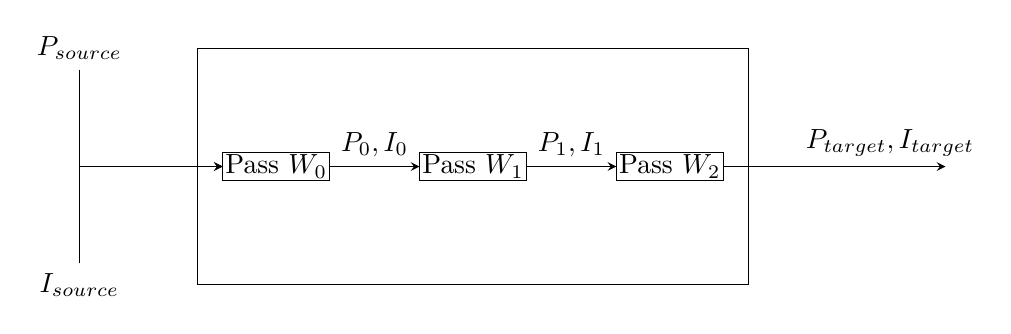
\begin{tikzpicture}
    \node [] (v01) at (-5,2.5) {$P_{source}$};
    \node [] (v02) at (-5,-0.5) {$I_{source}$};
    \node [bordered] (v1) at (-2.5,1) {Pass $W_0$};
    \node [bordered] (v2) at (0,1) {Pass $W_1$};
    \node [bordered] (v3) at (2.5,1) {Pass $W_2$};

    \draw [arrow] (v1) -- (v2) node[midway,above] {$P_0,I_0$};
    \draw [arrow] (v2) -- (v3) node[midway,above] {$P_1,I_1$};
    \draw [arrow] (v3) -- (6,1) node[near end,above] {$P_{target},I_{target}$};
    \draw [arrow](v01) -- (-5,1) -- (v1);
    \draw [arrow](v02) -- (-5,1) -- (v1);
    \draw [arrow] (-3.5,2.5) rectangle (3.5,-0.5);
  \end{tikzpicture}
  \end{mdframed}
  \caption{Overall architecture}
  \label{fig:arch2}
\end{figure}

To obtain this result, the existing optimizations are modified in two ways. First, transformation passes are built to understand the annotations passed externally and use them to optimize the code. The annotation are written in a FOL-like language that the optimizer can use. A \emph{Witness Generator} is built for every optimization; the witness Generator generates a \emph{witness} that can be proved independently to check the validity of the transformation (Figure~\ref{fig:arch1}).

\begin{figure}[b]
  \begin{mdframed}
  \centering
  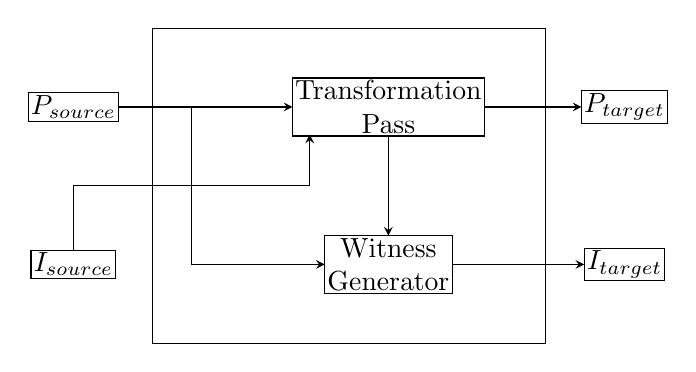
\begin{tikzpicture}
    \draw  (-4,2.5) rectangle (1,-1.5);
    \node [bordered] (v2) at (-1,1.5) {Transformation\\Pass};
    \node [bordered] (v3) at (-1,-0.5) {Witness\\Generator};
    \node [bordered] (v1) at (-5,1.5) {$P_{source}$};
    \node [bordered] (v5) at (2,1.5) {$P_{target}$};
    \node [bordered] (v4) at (-5,-0.5) {$I_{source}$};
    \node [bordered] (v6) at (2,-0.5) {$I_{target}$};
    \draw [arrow] (v1) edge (v2);
    \draw [arrow] (v2) edge (v3);
    \draw [arrow] (v4) -- (-5,0.5) -- (-2,0.5) -- (-2,1.15);
    \draw [arrow] (v1) -- (-3.5,1.5) -- (-3.5,-0.5) -- (v3);
    \draw [arrow] (v2) edge (v5);
    \draw [arrow] (v3) edge (v6);
  \end{tikzpicture}
  \end{mdframed}
  \caption{Witness-generating optimization pass}
  \label{fig:arch1}
\end{figure}

The approach for generating the witness is to set a \emph{stuttering simulation} relation between source and target programs. Stuttering simulation, as defined in \cite{namjoshi1997simple}, in this context comes more useful than regular strict simulation, as the target program may have fewer instructions than the source. It is shown \cite{zuck2005translation} that establishing a stuttering simulation relation from target to source is a sound and complete method for proving correctness, as opposed to strict simulation.

The framework is built open the Low-Level Virtual Machine compiler(LLVM). The choice is driven by the fact that LLVM represent a state of the art, modern, modular compiler, with a well maintained and documented codebase. LLVM optimization passes work on an intermediate language called \emph{LLVM Intermediate Representation} (IR), as presented in \cite{lattner2004llvm}. The IR is a Static Single Assignment (SSA) based representation that provides type safety, low-level operations, flexibility, and the capability of representing ``all'' high-level languages cleanly. It is the common code representation used throughout all phases of the LLVM compilation strategy.

This work is structured as follows. Chapter~\ref{cha:transformation_witness} introduces the concepts of witness and invariant propagation. They will be analyzed from a formal point of view, and some key properties of the witness are demonstrated. It is described that stuttering simulation is a sound and complete witness relation for generic code transformation, and that the very witness relation can be used to propagate the invariants. In Chapter~\ref{cha:witness_for_common_optimizations} the theoretical concepts shown previously are applied to some common optimizations in order to exemplify the critical points. For every optimization presented, a corresponding witness is described. In Chapter~\ref{cha:hacking_llvm} the LLVM framework design is presented and the key details in the implementations are described. It also describes how the transformations presented in the previous chapter are implemented. Chapter~\ref{cha:conclusions} describes the results obtained by the framework and the goals that will be pursued in the future, as well as provide with a conclusive overview of the work, comparing it to some related researches, and it introduces the limitation of the current framework, and how it can be extended.


	% \chapter{Formal methods and static optimization: a new approach}
	% 	\label{cha:formal_methods_and_static_optimization_a_new_approach}
	% 	% !TEX root =  ../thesis.tex

\section{Exploiting First Order Logic}
\label{sec:exploiting_first_order_logic}

\section{Solvers and Provers}
\label{sec:solvers_and_provers}

\section{Optimization}
\label{sec:optimization}


	% \chapter{Annotation language}
	% 	\label{cha:annotation_language}
	% 	% !TEX root =  ../thesis.tex

\section{ACSL}
\label{sec:acsl}

\subsection{Subsets of ACSL}
\label{sub:subsets_of_acsl}

\subsection{Grammar}
\label{sub:grammar}


	\chapter{The Transformation Witness}
		\label{cha:transformation_witness}
		% !TEX root =  ../thesis.tex

\section{Introduction}
\label{sec:theory_introduction}

To carry the annotations from the source program to the target, a \emph{witness relation} is built for every transformation. The generated witness is also used to check the correctness of the transformation, since it can be verified independently from the transformation. This makes the witness a very convenient and powerful abstraction, because proving its correctness is simpler than proving the formal correctness of a transformation, that is generally very complex. In a modern compiler, for example, even the simplest transformation can be made up of thousands of line of code. Witnessing a transformation is a new idea in the field of formal methods and compilers, and as such, it needs a formal definition that can be used in the theorems and hypotheses about its properties. From a theoretical point of view, the layout of witness generation is simple, yet, defining and proving its completeness requires some non-trivial demonstrations. In this chapter the concept of \emph{stuttering simulation} is also introduced, and it is shown that establishing a stuttering simulation relation from target to source is a sound and complete method for proving correctness.

The theory that is being presented inside this chapter was developed by Zuck and Namjoshi, in the paper called ``Witnessing Program Transformations''\cite{zucknamjoshi}. A briefer approach is given in \cite{namjzucktag}, where the results of this work are summarized.
% In this paper the theory behind the approach of witnessing the transformation is developed for the first time. The definitions that described the mathematical concepts are introduced, the theorems regarding the witness are expressed and a demonstration is laid out for almost all of them. This work draws from that paper the theory that is needed to build the framework implementation. Trying to define a new theory is far from the scope of this work, that instead aims at designing a framework and implementing it, based on the theory presented in this chapter. In some cases, however, the format of the mathematical object is modified in order to be consistent to the implementation, where the theory is manipulated in different ways for different reason (implementation, optimality, easiness of use). Clearly the new reformulation doesn't jeopardize the theoretical conclusions obtained with the original definition presented in the paper. Where it's possible the theorem formulation is taken as the same, in order not to lose formal correctness, and the demonstrations are not presented. For the formal demonstrations one can refer to the paper previously mentioned.

% In Chapter~\ref{cha:witness_for_common_optimizations} the idea of witness is applied to some common optimizations, to illustrate some features of witness generation. Subsequently, In Chapter~\ref{cha:hacking_llvm} the same problem is approached from the implementation side: a witness generator implementation is designed, and some witness-enhanced transformations are built for the LLVM Compiler, and which problems and difficulties have to be considered in order to build a correct implementation.

\section{Definitions}
\label{sec:definition}

The definitions presented in this section are basically the one used in \cite{zucknamjoshi}, with some minor changes to fit the implementation.

% In order to write the formal definition of witness, first some preliminary concepts need to be defined, which will be used later on to demonstrate useful properties of the witness relation. These definitions follow an incremental approach, That will end with the demonstration of these concepts in relation to some concrete transformation passes.

\begin{fdefinition}[Program]
\label{def:program}
A program is described as a tuple $(V, G, T, I)$, where
\begin{itemize}
  \item $V$ is a finite set of (typed) variables
  \item $G$ is a finite directed graph (it can be, for example, the control-flow graph)
  \item $T$ is a function specifying, for every edge $(i, j) \in G$, a symbolic transition condition denoted $T_{i,j}(V, V')$. Primed variables are used to denote the value of the program variables at the program state after the transition
  \item $I(V)$ is an initial condition for the program
\end{itemize}
\end{fdefinition}

\begin{figure}[ht]
  \begin{mdframed}
  \vspace{1cm}
  \centering
  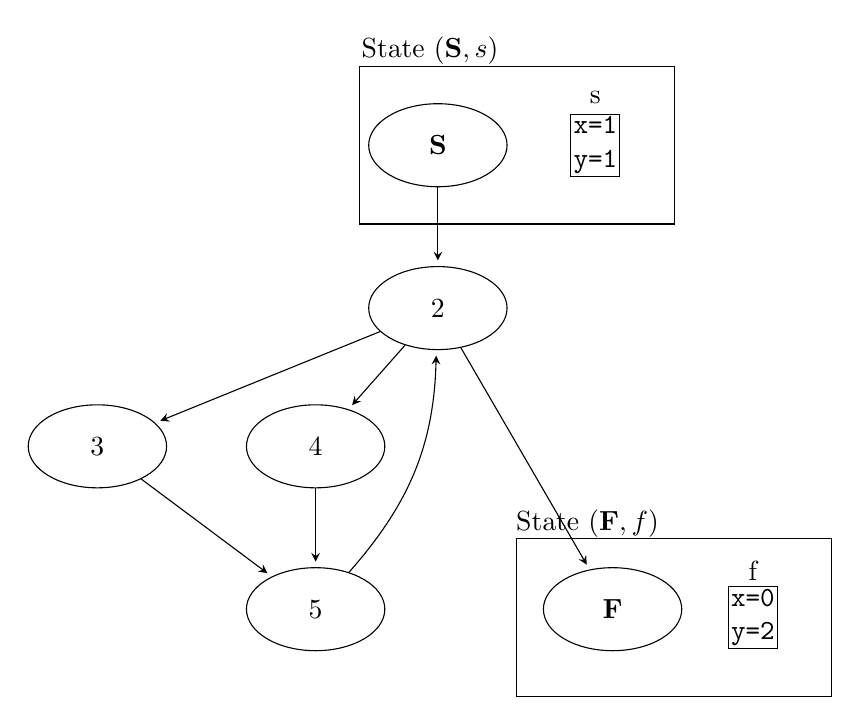
\begin{tikzpicture}[%
    ->,
    shorten >=2pt,
    >=stealth,
    node distance=1cm,
    noname/.style={%
      ellipse,
      minimum width=5em,
      minimum height=3em,
      draw}
    ]
  \node[noname] (1) {\textbf{S}};
  \node[noname] (2) [below=of 1] {2};
  \node[noname] (4) [node distance=1cm and 3mm,below left=of 2] {4};
  \node[noname] (3) [left=of 4] {3};
  \node[noname] (5) [below=of 4] {5};
  \node[noname] (6) [node distance=2cm,right=of 5] {\textbf{F}};
  \path (1) edge node{} (2)
        (2) edge node{} (3)
        (2) edge node{} (4)
        (2) edge node{} (6)
        (3) edge node{} (5)
        (4) edge node{} (5)
        (5) edge [bend right=20pt] node {} (2);
  \node [bordered] at (2,0) {\texttt{x=1}\\\texttt{y=1}};
  \node [bordered] at (4,-6) {\texttt{x=0}\\\texttt{y=2}};
  \draw  (-1,1) rectangle (3,-1);
  \draw  (1,-5) rectangle (5,-7);
  \node [] at (2,0.6) {s};
  \node [] at (4,-5.4) {f};
  \node [] at (-0.1,1.2) {State $(\textbf{S},s)$};
  \node [] at (1.9,-4.8) {State $(\textbf{F},f)$};
  \end{tikzpicture}
  \vspace{1cm}
  \end{mdframed}
  \caption[Example of graph $G$]{Example of graph $G$. A pair $(l,v)$ is a \emph{state}. State $(\textbf{S},s)$ is \emph{initial}, State $(\textbf{F},f)$ is \emph{final}}
  \label{fig:programcfg}
\end{figure}

Every transition relates current and next-state values of the variables. $G$ has two distinguished nodes, $\textbf{S}$ and $\textbf{F}$. The $\textbf{S}$ node has no incoming edges, and the $\textbf{F}$ node has no outgoing edges, meaning that from $F$ no transition can be triggered (see Figure~\ref{fig:programcfg}). In this work we assume that every program P is deadlock-free, meaning that only the node $\textbf{F}$ has no enabled outgoing transition.
% A further assumption is that the program is not guaranteed to terminate, i.e., it can reach  $\textbf{F}$ from any node. In this case the program computation starves.

A \emph{state} of a program is given by a pair $(l, v),$ where $l$ is a node of $G$ and $v$ is type-consistent assignment of values to each variable in $V$. A state is defined as \emph{initial} if and only if $ l = \textbf{S} \land I(v)$ holds.
% A state such that $ l = \textbf{S} \land !I(v)$ is an invalid initial state for the program.
A state is \emph{final} if and only if $ l = \textbf{F}$.

A transition system can be defined w.r.t. the program definition as follows.

\begin{fdefinition}[Transition System]
A transition system $T$ is given by a tuple $(S,I,R)$ where:

\begin{itemize}
  \item $S$ is a set of states,
  \item $I$ is the subset of initial states (i.e. inputs),
  \item $R \subseteq S \times S$ is a transition relation
\end{itemize}
\end{fdefinition}

A program $P(V, G, T, I)$ (as definied in Definition~\ref{def:program}) induces the transition system where the states are interpretations of $V$, the initial states are the those in $I$, and the relation $R$ is that defined symbolically by $T$. Using the definition of transition system instead of the program in the simulation definition will simplify them, without losing generality.

Moreover, a \emph{program computation} of lenght $n$ is a sequence of states $s_0, s_1 ,\ldots s_n$ where $s_0$ is initial and for each pair $s_i=(l_i,v_i), s_{i+1}=(l_{i+1},v_{i+1})$ of consecutive states on the sequence, $(l_i, l_i+1)$ is an edge in $G$, and the transition condition $T_{i,i+1}(v_i,v_i+1)$ holds.

A computation can have infinite length. A computation is \emph{terminating} if $s_n = (\textbf{F},v_n)$. A computation is \emph{maximal} when no transition can be enabled from the last state, i.e., when it's terminating or infinite.

\begin{fdefinition}[State Matching]
Let $T$, $S$ be two programs and $T_T(S_T,I_T,R_T)$,$T_S(S_S,I_S,R_S)$ the corresponding transition relations. States $t \in S_T$ and $s \in S_S$ match, denoted $t \simeq s$, if $t$ and $s$ assign the same value to every variable $v \in V' = V_S \cap V_T$.
\end{fdefinition}

\begin{fdefinition}[Path Matching]
\label{def:path_matching}
For Programs $T$ and $S$ a maximal computation $\tau$ of program $T$ is \emph{matched} by a maximal computation of $\sigma$ of program $S$ if the following conditions all hold:
\begin{itemize}
  \item The starting state of $T$ and $S$ match
  \item if $(\textbf{F}_T,v) \in \tau$ for some variable assignment $v$, then for some $w$, $(\textbf{F}_S,w) \in \sigma$
  \item if $\sigma$ has no final state, neither does $\tau$
\end{itemize}

% The second and third conditions can be equivalently substituted by the following condition: $(\textbf{F}_T,v) \in \tau \iff (\textbf{F}_S,w) \in \sigma$.

\end{fdefinition}

\begin{fdefinition}[Implementation]
Given two programs, $T$ and $S$, $T$ \emph{implements} $S$ if for every maximal computation $\tau$ of $T$, there is a maximal computation $\sigma$ of $S$ that matches it.
\end{fdefinition}

If $T$ implements $S$, then every terminating computation of $T$ has a corresponding terminating computation of $S$ starting from a matching initial state such that the final states (if any) also match. Hence, the input-output relation of $T$ is included in that of $S$, w.r.t. the common variables. Moreover, if $T$ has a non-terminating computation from some initial state, non-termination is also possible for $S$ from a matching state. This disallows, for example, pathological ``implementations'' where $T$ has no terminating computations, so that the input-output relation of $T$ (the empty set) is trivially contained in the input-output relation of $S$.

\begin{fdefinition}[Transformation Function]
A \emph{transformation} is a \emph{partial} function on the set of programs. A transformation $\delta$ is \emph{correct} if for every program $S$ in its domain, $T=\delta (S)$ implements $S$.
\end{fdefinition}

In practical terms, a transformation is partial because it needs not to apply to all programs. Indeed, much of the effort in compiler optimization is on the analysis required to determine whether a particular transformation can be applied. This is a very important point, that enforces the idea that, from a theoretical point of view, verifying the witness is much easier than verifying the whole transformation. It should be remembered also that the witnessing approach doesn't try to verify the correctness of the transformation over all legal inputs. As translation validation approach \cite{pnueli1998translation}, the witness aims at verifying that an instance of transformation produced an output that implements the input.

\section{Simulation relations}
\label{sec:stuttering_simulation}

Now we introduce two different kind of transition relations: Step and Stuttering Simulation. Both of them can be used as witness format, since, as it will be pointed out below, both can guarantee that the target program is a correct implementation of the source. The basic difference between the two relations is in terms of the kind of transformation that can be witnessed. A proof of the properties of the simulation is sketched but not formally expressed. The complete demonstrations are laid out in \cite{zucknamjoshi}.

\begin{fdefinition}[Step Simulation]
Given the transition systems $T$ and $S$, a relation $X \subseteq S_T \times S_S$ is a \emph{step simulation} if:
\begin{itemize}
  \item the domain of $X$ includes all initial states of $T$
  \item for any $(t,s) \in X$, $t$ and $s$ satisfy the same propositions and for every $t'$ such that $t,t' \in R_T$, there is a $s'$ such that $(s,s') \in R_S$ and $(t',s') \in X$.
\end{itemize}
\end{fdefinition}

It is shown in \cite{zucknamjoshi} that step simulation guarantees that the target program is a correct implementation of the source:

\begin{ftheorem}[Step Soundness\cite{zucknamjoshi}]
\label{thm:step_soundness}
  For programs $T$ and $S$, $T$ implements $S$ if there is a step simulation $X(S_S\times S_T)$ from the states of every $T$-computation to the states of $S$-computation such that:
  \begin{itemize}
    \item for every initial state $s_{T}$ of $T$ there is an initial state $s_{S}$ such that $(s_{T},s_{S}) \in X$
    \item for every final state $t_{T}$ of $T$, if  $(t_{T},t_{S}) \in X$ then $t_{S}$ is a final state of $S$
  \end{itemize}
\end{ftheorem}
Thus, checking the single-transition conditions of step simulation, together with the two additional conditions of Theorem~\ref{thm:step_soundness}, is enough to show that $T$ implements $S$. These checks can be encoded as correctness questions and resolved with an automatic decision procedure.

However, it is not always possible to draw a transition relation between a correctly implemented target and its source program. In fact, if a step simulation relation can be defined, for every step taken in the target transition, there is a corresponding step in the source transition. This obviously requires the two transitions to have the same exact length.

Stuttering Simulation Relation, the next witness format that is described, relaxes this exact, 1-1 matching by permitting $\tau$ and $\sigma$ to be matched in segments, as illustrated in Figure~\ref{fig:stuttering1}.

\begin{figure}[hb]
  \begin{mdframed}
  \vspace{1cm}
  \centering
  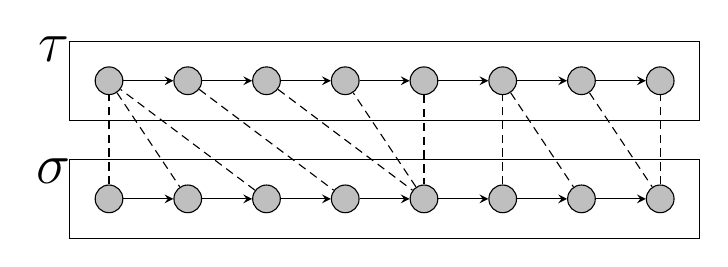
\begin{tikzpicture}
  \node [gcircle] (v) at (-2.5,1.5) {};
  \node [gcircle] (v1) at (-1.5,1.5) {};
  \node [gcircle] (v2) at (-0.5,1.5) {};
  \node [gcircle] (v3) at (0.5,1.5) {};
  \node [gcircle] (v4) at (1.5,1.5) {};
  \node [gcircle] (v5) at (2.5,1.5) {};
  \node [gcircle] (v6) at (3.5,1.5) {};
  \node [gcircle] (v7) at (4.5,1.5) {};
  \node [gcircle] (v8) at (-2.5,0) {};
  \node [gcircle] (v9) at (-1.5,0) {};
  \node [gcircle] (v10) at (-0.5,0) {};
  \node [gcircle] (v11) at (0.5,0) {};
  \node [gcircle] (v12) at (1.5,0) {};
  \node [gcircle] (v13) at (2.5,0) {};
  \node [gcircle] (v14) at (3.5,0) {};
  \node [gcircle] (v15) at (4.5,0) {};
  \draw [densely dashed] (v8) edge (v);
  \draw [densely dashed] (v) edge (v9);
  \draw [densely dashed] (v10) edge (v);
  \draw [densely dashed] (v1) edge (v11);
  \draw [densely dashed] (v2) edge (v12);
  \draw [densely dashed] (v12) edge (v3);
  \draw [densely dashed] (v4) edge (v12);
  \draw [densely dashed] (v5) edge (v14);
  \draw [densely dashed] (v13) edge (v5);
  \draw [densely dashed] (v15) edge (v7);
  \draw [densely dashed] (v6) edge (v15);
  \draw [arrow] (v) edge (v1);
  \draw [arrow] (v1) edge (v2);
  \draw [arrow] (v2) edge (v3);
  \draw [arrow] (v3) edge (v4);
  \draw [arrow] (v4) edge (v5);
  \draw [arrow] (v5) edge (v6);
  \draw [arrow] (v6) edge (v7);
  \draw [arrow] (v8) edge (v9);
  \draw [arrow] (v9) edge (v10);
  \draw [arrow] (v10) edge (v11);
  \draw [arrow] (v11) edge (v12);
  \draw [arrow] (v13) edge (v14);
  \draw [arrow] (v12) edge (v13);
  \draw [arrow] (v14) edge (v15);
  \draw  (-3,2) rectangle (5,1);
  \node [] at (-3.2,1.9) {\huge{$\tau$}};
  \draw  (-3,0.5) rectangle (5,-0.5);
  \node [] at (-3.2,0.35) {\huge{$\sigma$}};
  \end{tikzpicture}
  \vspace{1cm}
  \end{mdframed}
  \caption{Stuttering Simulation}
  \label{fig:stuttering1}
\end{figure}

It has been demonstrated\cite{namjoshi1997simple} that the segments can be replaced by single steps, adding an additional dimension to the stuttering simulation relation. This is done by adding a \emph{ranking function} $Rank: (T,S) \rightarrow \mathbb{N}$ which decreases strictly at each stuttering step. In this work a simpler form of stuttering simulation is necessary.

\begin{figure}[ht]
  \begin{mdframed}
  \vspace{1cm}
  \centering
  \begin{subfigure}[b]{0.3\textwidth}
    \centering
    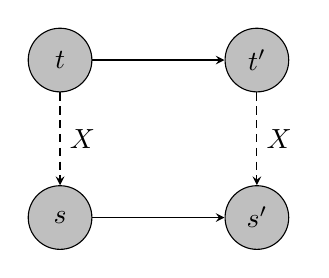
\begin{tikzpicture}
    \node [gcircle, minimum size = 23] (u) at (-2.5,2) {$t$};
    \node [gcircle, minimum size = 23] (u1) at (0,2) {$t'$};
    \node [gcircle, minimum size = 23] (v) at (-2.5,0) {$s$};
    \node [gcircle, minimum size = 23] (v1) at (0,0) {$s'$};

    \draw [densely dashed, arrow] (u) edge node[midway,auto] {$X$} (v);
    \draw [densely dashed, arrow] (u1) edge node[midway,auto] {$X$} (v1);

    \draw [arrow] (v) edge (v1);
    \draw [arrow] (u) edge (u1);
    \end{tikzpicture}
    \caption{Case 1}
    \label{fig:stuttering21}
  \end{subfigure}
    \begin{subfigure}[b]{0.3\textwidth}
    \centering
    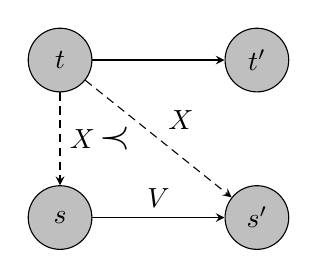
\begin{tikzpicture}
    \node [gcircle, minimum size = 23] (u) at (-2.5,2) {$t$};
    \node [gcircle, minimum size = 23] (u1) at (0,2) {$t'$};
    \node [gcircle, minimum size = 23] (v) at (-2.5,0) {$s$};
    \node [gcircle, minimum size = 23] (v1) at (0,0) {$s'$};

    \draw [densely dashed, arrow] (u) edge node[midway,auto] {$X$} (v);
    \draw [densely dashed, arrow] (u) edge node[midway,auto] {$X$} (v1);

    \draw [arrow] (v) edge node[midway,auto] {$V$} (v1);
    \draw [arrow] (u) edge (u1);
    \node at (-1.8,1) {\Large{$\prec$}};
    \end{tikzpicture}
    \caption{Case 2}
    \label{fig:stuttering22}
  \end{subfigure}
    \begin{subfigure}[b]{0.3\textwidth}
    \centering
    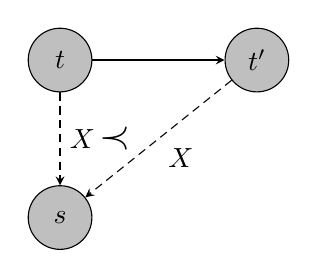
\begin{tikzpicture}
    \node [gcircle, minimum size = 23] (u) at (-2.5,2) {$t$};
    \node [gcircle, minimum size = 23] (u1) at (0,2) {$t'$};
    \node [gcircle, minimum size = 23] (v) at (-2.5,0) {$s$};

    \draw [densely dashed, arrow] (u) edge node[midway,auto] {$X$} (v);
    \draw [densely dashed, arrow] (u1) edge node[midway,auto] {$X$} (v);

    \draw [arrow] (u) edge (u1);
    \node at (-1.8,1) {\Large{$\prec$}};
    \end{tikzpicture}
    \caption{Case 3}
    \label{fig:stuttering23}
  \end{subfigure}
  \vspace{1cm}
  \end{mdframed}
  \caption{Stuttering Simulation with ranking}
  \label{fig:stuttering2}
\end{figure}

\begin{fdefinition}[Stuttering Simulation with Ranking function]
\label{def:stuttering_simulation}
Given Transition systems $B$ and $A$, a relation $ X \subseteq S_T \times S_S $ augmented with a partial ranking function, $Rank: (S_T,S_S) \rightarrow \mathbb{N}$, over a well-founded domain $(\mathbb{N},\prec)$, is a \emph{stuttering simulation} if:
\begin{itemize}
  \item the domain of $X$ includes all initial states of $T$ and
  \item for any $(t, s) \in X$, $t$ and $s$ satisfy the same propositions and for every $t'$ such that $(t,t') \in R_T$, one of the following holds:
  \begin{itemize}
    \item There is $s'$ such that $(s,s') \in R_S \land (t',s') \in X$ (Figure~\ref{fig:stuttering21}), or
    \item There is $s'$ such that $(s,s') \in R_S \land (t,s') \in X \land rank(t,s') \prec rank(t,s)$ (stuttering on A, Figure~\ref{fig:stuttering22}), or
    \item $(t',s) \in X$ and rank $(t',s) \prec (t,s)$ (stuttering on B, Figure~\ref{fig:stuttering23}).
  \end{itemize}
\end{itemize}
\end{fdefinition}

A graphical explanation of this definition is given in Figure~\ref{fig:stuttering2}. It is immediate to observe how step simulation is a specialization of stuttering simulation. If we define three sets $\mathcal{REL},\mathcal{STUT},\mathcal{STEP}$ as the set of all general relations, step simulation relations and stuttering simulation relations respectively, we have $\mathcal{STEP} \subset \mathcal{STUT} \subset \mathcal{REL}$ (Figure~\ref{fig:relations}). This result will help to clarify some considerations. While $\mathcal{REL}$ can define every transformation relation from program $A$ to $B$, not all are correct (i.e, $B=X(A)$ implements $A$). On the other hand, this is true for all the step simulations (Theorem~\ref{thm:step_soundness}), yet, as already stated before, step simulation is too restrictive in terms of transformations that can be simulated. In fact, it can be applied only when the the transformation doesn't rearrange, eliminate or add instructions. Therefore, stuttering simulation is the best candidate to accommodate all kind of transformations, as it is, we'll observe, a sound and complete simulation. It must be considered also that the definition of stuttering simulation adds an additional dimension to the relation, that is the one defined by the ranking function that accompanies the stuttering simulation to guarantee that the lengths of the matched segment are finite. The figure doesn't take into account the ranking function, so it is a simplification of the actual property of stuttering simulation. In fact, as it is shown in \cite{zucknamjoshi}, without the ranking function it wouldn't be possible to demonstrate the completeness of the stuttering simulation.

\begin{figure}[ht]
  \begin{mdframed}
    \vspace{1cm}
    \centering
    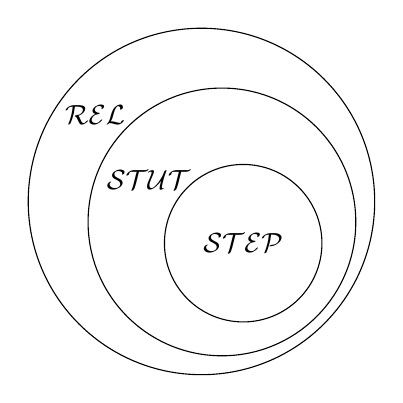
\begin{tikzpicture}
      \def\firstcircle{(0:0) circle (2.2cm)}
      \def\secondcircle{(0.26,-0.26cm) circle (1.7cm)}
      \def\thirdcircle{(0.53,-0.53cm) circle (1cm)}
      \draw \firstcircle node[above left = 1.2cm] {$\mathcal{REL}$};
        \draw \secondcircle node [above left = .4cm] {$\mathcal{STUT}$};
        \draw \thirdcircle node [] {$\mathcal{STEP}$};
    \end{tikzpicture}
    \vspace{1cm}
  \end{mdframed}
  \caption{Relation hierarchy}
  \label{fig:relations}
\end{figure}

\begin{ftheorem}[Soundness\cite{zucknamjoshi}]
\label{thm:soundness}
Let $X$ be a stuttering simulation relating states of a program $T$ to those of program $S$. Then $T$ is a correct implementation of $S$ when the following conditions all hold:
\begin{itemize}
  \item For every initial state $s$ of $S$, there is an initial state $t$ of $T$ such that $(t, s) \in X $ and $ t \simeq s$.
  \item Final states of $S$ or $T$ are $X$-related to only final states of the other program. Moreover, if $t$ and $s$ are $X$-related final states of $T$ and $S$, then $t \simeq s$.
\end{itemize}
\end{ftheorem}

The conditions expressed in the soundness theorem gives the definition of \emph{Witness Relation}:

\begin{fdefinition}[Witness]
Let $S$ and $T$ be programs related by a stuttering simulation relation $W$ from the state space of $T$ to that of $S$. $W$ is a \emph{Witness relation} if the soundness conditions hold:
\begin{itemize}
  \item For every initial state $u$ of $T$, there is an initial state $v$ of $S$ such that $(u,v) \in W $ and $ u \simeq v$.
  \item Final states of $S$ or $T$ are $W$-related to only final states of the other program. Moreover, if $u$ and $v$ are $W$-related final states of $T$ and $S$, then $u \simeq v$.
\end{itemize}
In other words, that means that the stuttering simulation is a sound witness.
\end{fdefinition}

Based on Manolios\cite{manolios2003compositional}, Namjoshi and Zuck proved that stuttering simulation is sound and complete.
 % when augmented with history and prophecy variables, where prophecy variables are used only to overcome non-determinism. A specialization of Manolios' result is shown for programs where transitions are deterministic and the only non-determinism is the choice of initial state. In this specialization prophecy variables are unnecessary; moreover, w.r.t. to this work the history can be assumed by the definition of stuttering simulation. In practice, this is not a limitation, because internal representation of the compilers are statically deterministic.

% The following theorem has a very important result, because it shows that is always possible, at least in theory, to generate a witness, whatever transformation has occurred and whatever was the source program. The guarantee of completeness is a result that Translation Validation techniques lacks, as TV is applicable only to a certain set of transformation, and the proof is not guaranteed to be always found (\cite{zuck2005translation}).

% \begin{ftheorem}[Completeness]
% \label{thm:completeness}
% Consider programs $B$ and $A$ both of which have a deterministic transition relation. If $B$ refines $A$, there is a stuttering simulation relation between the programs augmented with history variables which meets the conditions of Theorem~\ref{thm:soundness}(Soundness Theorem).
% \end{ftheorem}

\section{Invariant propagation}
\label{sec:invariant_propagation}

A relation that satisfies the Witness format can also be used to ``propagate'' the assertions from end to end of the transformation pass, making the additional transformation to be used also in different part of the transformation process, rather than just by the first one. This result of this property is what the second problem pointed out in the introductory section. \emph{Propagation} informally means that if an assertion $\theta$ is true for a subset of source states $S_S' \in S_S$, the propagated assertion $\theta'$ must be true for all and only the target states $S_T' \in S_T$ where every state $t \in S_T'$ is related to some state $s \in S_S'$ by the witness relation $W$. Now a more formal description will be provided.

First we define the concept of pre-image of $\theta$ under $W$, denoted ($\langle W \rangle \theta$), as the set $\left\{(m,t) | (\in l,s : ((m,t),(l,s)) \in W \land \theta(l,s)\right\}$. The following theorem holds:

\begin{ftheorem}[Invariant Propagation\cite{zucknamjoshi}]
\label{thm:propagation}
Let $W$ be a stuttering simulation witness for a transformation from program $T$ to program $S$. If $\theta$ is an invariant for $S$, the set $\langle W \rangle \theta$ is an invariant for $T$. Moreover, if $\theta$ is inductive, so is $\langle W \rangle \theta$.
\end{ftheorem}
The sketch of the proof for the correctness of  $\langle W \rangle \theta$ as invariant at Target is as follows. Let $\theta$ be an invariant holding for every state of a program $S$. For every valid computation $\tau$ of program $T$, there must exist, from the definition of witness relation, a computation $\sigma$ of program $S$ such that $\forall t \in \tau, \exists s \in \sigma, W(t, s)$. It is true also that $\forall s \in \sigma, s \in \theta$. The last formula holds because $\sigma$ is a computation of S (where $\theta$ holds). Combining the last two formulas ensues that $\underset{t \in \tau}{\bigcup} \in \langle W \rangle \theta$. Hence, $\langle W \rangle \theta$ is a correct invariant for program $T$.

\section{Generalization}
\label{sec:generalization}
The transition relation can be generalized and adjusted to the concept of control-flow graph (CFG) of a program $P$. In this generalization, the states of a program refers only to the beginning of a basic block of the graph, and the transition relation maps every node of the CFG of the program to its successors. Hence, every transition can cover more than one instruction. The generalization is useful for two different reasons. This restricts the cases where step simulation is not sufficient and stuttering simulation is necessary,
% making the generation of the witness easier for these cases.

Consider the example of Dead Code Elimination. As it will be shown in the following chapter, DCE transformation can be witnessed by a stuttering simulation relation. However, if we generalize the transition relation to work over the basic blocks rather than single instructions, step simulation is sufficient to prove the correctness of this transformation. This is due to the fact that Dead code elimination doesn't change the CFG structure. Hence, it follows that stuttering simulation is usually necessary when the transformation reorders, eliminates, or add nodes of the Control Flow Graph.

The second reason is that many compilers, such as LLVM, build the CFG of the function as a preliminary step before every optimization pass. This implies that building the generalized relations over the existing CFG is a more efficient approach than building instruction-wise transitions.


	\chapter{Witness for Common Optimizations}
		\label{cha:witness_for_common_optimizations}
		% !TEX root =  ../thesis.tex

In this Chapter the witnesses for several standard optimizations are defined. These optimizations are chosen for their commonality and in order to illustrate features of the witness generation. We consider constant propagation, dead code elimination, control-flow graph compression and loop optimizations. Some transformation can be witnessed with a simple step simulation, however other transformations require the simulation to be stuttering, as the transformation can result in the target being shorter or longer than the source. As a side result of the examples, it is shown that the analysis required to check if a transformation can be triggered is more difficult than the witness generation procedure, showing that witness generation can be, in theory, an efficient transformation checker. Witness generation, essentially, makes explicit the implicit invariants gathered during the analysis. These examples confirm also the concept that, from a theoretical point of view, a witness can be generated for every kind of optimization, even though the complexity of the optimization will impact on the complexity of the witness. The examples are taken from \cite{zucknamjoshi}, and modified to highlight the details that this chapter wants to stress out.

The actual implementation for some of these transformations will be exposed in Chapter~\ref{cha:hacking_llvm}. Therefore all the details concerning the implementation will be put aside, in order to focus on the key concepts both of witness generation and invariant propagation.

\section{Constant Propagation}
\label{sec:constant_propagation_th}

In the \emph{Constant Propagation} pass, the analysis checks if any variable has a static assigned constant value. In the example of Figure~\ref{fig:constprop_th} all the values are constant-folded up.

\begin{figure}[t]
  \begin{mdframed}
  \centering
  \begin{subfigure}[t]{0.49\textwidth}
    \centering
    \begin{lstlisting}
L1: x = 1+2;
L2: y = x+x;
L3: y = y+1;
L4: x = y;
    \end{lstlisting}
    \caption{Source}
    \label{fig:sconstprop_th}
  \end{subfigure}
  \begin{subfigure}[t]{0.49\textwidth}
    \centering
    \begin{lstlisting}
L1: x = 3;
L2: y = 6;
L3: y = 7;
L4: x = 7;
    \end{lstlisting}
    \caption{Target}
    \label{fig:tconstprop_th}
  \end{subfigure}
  \end{mdframed}
  \caption{Constant propagation example}
  \label{fig:constprop_th}
\end{figure}

The witness generation for constant propagation basically draws from the invariants generated during the analysis. The invariant, called $constant(l)$, simply describes the set of variables that have a statically computed constant value at location $l$. For example, the invariant at \texttt{L3} is $x =3 \land y = 6$.

The witness relation is expressed in a symbolic form. The general shape of the relation for constant propagation is the following: a target state $(m, t)$ is related to a source state $(l, s)$ if and only if:
\begin{itemize}
  \item labels are identical (i.e., $m = l$),
  \item variables have identical values (i.e., for every variable $x, s(x) = t(x)$), and
  \item variables in the source system have values given by their invariant (i.e., $constants(l)$ holds at $s$)
\end{itemize}
Where for every variable $x$ in the source, $\bar{x}$ indicates its corresponding version in the target. For example, in symbolic form, the relation includes the clause
\[
  @L3 \land @\bar{L3} \land (x = \bar{x}) \land (y = \bar{y}) \land (z = \bar{z}) \land x = 3 \land y = 6
\]

It's necessary that the invariants hold at the source location, because this establishes the correspondence between target and source. For instance, the transition from $L2$ to $L3$ is matched by the transition from $\bar{L2}$ to $\bar{L3}$ only because the value of $x$ is defined as constant in $constant(L2)$

\section{Dead Code Elimination}
\label{sec:dce_and_cfgc_th}

Dead code elimination analyzes the code, building use-define chains for every assignment instruction, and marks all those instructions for which use set is empty. This means that the assigned value is not being used in any of the program computation and removing it doesn't change the semantics of the code. In this context, dead code elimination is split in two separate phases, the second being a restrictd instance of control flow graph compression. If the transition from location $m$ to location $n$ assigns a value to a variable $v$ that is dead (i.e., not live) at $n$, this assignment may be replaced with a skip statement. This is illustrated in Figure~\ref{fig:dce_th} which performs dead-code detection for the output of the constant propagation analysis. The result of the liveness analysis is a set, denoted $live(l)$, for each location $l$ of the source program.

\begin{figure}[t]
  \begin{mdframed}
  \centering
  \begin{subfigure}[t]{0.49\textwidth}
    \centering
    \begin{lstlisting}
L1: x = 3;
L2: y = 6;
L3: y = 7;
L4: x = 7;
    \end{lstlisting}
    \caption{Source}
    \label{fig:sdce_th}
  \end{subfigure}
  \begin{subfigure}[t]{0.49\textwidth}
    \centering
    \begin{lstlisting}
L1: x = skip;
L2: y = skip;
L3: y = 7;
L4: x = 7;
    \end{lstlisting}
    \caption{Target}
    \label{fig:tdce_th}
  \end{subfigure}
  \end{mdframed}
  \caption{Dead code elimination example}
  \label{fig:dce_th}
\end{figure}

Here is described a general procedure for generating a witness for DCE. A target state $(m, t)$ is related to a source state $(l, s)$ if and only if:
\begin{itemize}
  \item labels are identical (i.e., $m = l$), and
  \item every variable that is live at $l$ has the same value as the corresponding variable at $m$. I.e., for every variable $x$ such that $x \in live(l): s(x) = t(x)$.
\end{itemize}
For example, in symbolic form, the relation includes the clause
\[
  @\bar{L4} \land @L4 \land (y = \bar{y})
\]
as only the variable $x$ is live at $L4$. For any correct dead code elimination transformation, the relation defined above is a strong simulation witness.

Continuing the example from the result of dead code elimination, the control flow graph has unnecessary \emph{skip} statements. These may be removed using the rewrite rule $skip; S \rightarrow S$, for any statement $S$. This compresses the control flow graph. Other instances of compression may occur in the following situations:
\begin{itemize}
  \item a sequence such as \texttt{goto L1; L1:S} is replaced with \texttt{L1:S}, or
\item the sequence \texttt{S1; if (C) skip else skip; S2} is replaced with \texttt{S1;S2}.
\end{itemize}
In all these cases the computation in the target is shorter than the one in the source,

The general witness definition relates a target state $(m,t)$ to a source state $(l,s)$ if $s = t$ and either $l = m$ or $l$ lies on a linear chain of \emph{skip} statements from $m$ in the source graph.

\begin{figure}[t]
  \begin{mdframed}
  \centering
  \begin{subfigure}[b]{0.49\textwidth}
    \centering
    \begin{lstlisting}
L1: x = skip;
L2: y = skip;
L3: y = 7;
L4: x = 7;
%*\vspace{0cm}
    \end{lstlisting}
    \caption{Source}
    \label{fig:scfgc_th}
  \end{subfigure}
  \begin{subfigure}[b]{0.49\textwidth}
    \centering
    \begin{lstlisting}
L3: y = 7;
L4: x = 7;
%*\vspace{0cm}
    \end{lstlisting}
    \caption{Target}
    \label{fig:tcfgc_th}
  \end{subfigure}
  \end{mdframed}
  \caption{Control-Flow-Graph compression example}
  \label{fig:cfgc_th}
\end{figure}

For a correct control-flow graph compression, the defined relation is a stuttering simulation witness. Moreover, as a result of the closure property for stuttering simulation, it is possible to take the witnesses for constant propagation $W_1$, dead-code elimination $W_2$, and control-flow graph compression $W_3$ and compose them to form a single witness $W = W_1;W_2;W_3$for the transformation from the program in Figure~\ref{fig:sconstprop_th} to the program in Figure~\ref{fig:tcfgc_th}.

\section{Reordering Transformations}
\label{sec:reordering_transformations}

A \emph{reordering transformation} is a program transformation that changes the order of execution of the code, without adding or deleting any statements. It preserves a dependence if it preserves the relative execution order of the source and target of that dependence, and thus preserves the semantical meaning of the program. Reordering transformations cover many loop optimizations, including fusion, distribution, interchange, tiling, and reordering of statements within a loop body.

A generic loop can be described, as introduced in \cite{zuck2005translation}, by the statement \texttt{for $i \in \mathcal{I}$ by $\prec_{\mathcal{I}}$ do B(i) } where $i$ is the loop induction variable and $\mathcal{I}$ is the set of the values assumed by $i$ through the different iterations of the loop. The set $\mathcal{I}$ can typically be characterized by a set of linear inequalities. While in \cite{zuck2005translation} ``structure preserving'' and ``Reordering'' transformation passes are treated differently, here we follow \cite{zucknamjoshi} and let the witness relation to be defined so that it allows for uniform treatment of the two types of transformations.

\section{Loop Invariant code motion}
\label{sec:a_simple_reordering_transformation}

\emph{Loop invariant code motion} (also referred to as ``hoisting'') moves some instructions from the inner to the outer body of a loop without affecting the semantics of the program. Usually a reaching definitions analysis is used to detect whether a statement or expression is loop invariant. For example, if all reaching definitions for the operands of some simple assignment are outside of the loop, the assignment can be moved out of the loop. Moreover, in order to move instructions outside the loop, LICM analysis must guarantee that there is at least one iteration for every different computation case of the program. See for example Figure~\ref{fig:licm_th} which is a simplified version of an example from \cite{steven1997advanced}. Since the loop is going to be executed at least once, the assignments to $a$ and $c$, which are not dependent on any statement in the loop body, can be moved outside of the loop.

\begin{figure}[t]
  \begin{mdframed}
  \centering
  \begin{subfigure}[b]{0.49\textwidth}
    \centering
    \begin{lstlisting}
L0: i = 1;
L1: while(i<100){
L2:   c = 3;
L3:   i = i + 1;
    }
    \end{lstlisting}
    \caption{Source}
    \label{fig:slicm_th}
  \end{subfigure}
  \begin{subfigure}[b]{0.49\textwidth}
    \centering
    \begin{lstlisting}
L0: i = 1;
L2: c = 3;
L1: while(i<100){
L3:   i = i + 1;
    }
    \end{lstlisting}
    \caption{Target}
    \label{fig:tlicm_th}
  \end{subfigure}
  \end{mdframed}
  \caption{Loop Invariant Code Motion example}
  \label{fig:licm_th}
\end{figure}

The transformation analyzer will detect the lack of dependencies of the statement in $L2$ on the other statements in the body, together with the fact that the loop is guaranteed to be executed at least once. The witness is generated in the following fashion. The simulation maps the first statements of the target program (In this case $L0$) and the first iteration of the target loop into the first iteration of the source loop. This mapping of course stutters, as there are more instructions in the target program segment than in the source program segment. Thus, the corresponding symbolic (stuttering simulation) will include the following clause: $L3 \land \bar{L3} \land i=\bar{i} \land c=\bar{c} \land c=3$. From the second iteration onwards, when $i>1$, the two loops are linked one by one in a stuttering simulation (since one target instruction in the target loop is mapped over two instructions in the source loop).

There is also a more general Loop invariant code motion that combines ``hoisting'' (where the instructions are moved before the loop body, as seen above) and ``sinking'' (where the instructions are moved after the loop body). For sinking, it must be checked that the moved instruction is not used inside the loop and that the loop is executed at least once. Given that, the witness generation follows the one described for the hoisting loop invariant code motion.


	\chapter{Design and Implementation}
		\label{cha:hacking_llvm}
		% !TEX root =  ../thesis.tex

In this chapter we describe the implementation of the theoretic transformations described in Chapter~\ref{cha:transformation_witness}: witness generation, witness checking and invariant propagation. The source code is available as a git repository\footnote{\url{https://bitbucket.org/itajaja/llvm-csfv}}. Basically it is a fork from the original LLVM repository where the additional passes and structures are being added. Description on how to run the program and basic examples are given in Appendix A.

We introduce an overview of the technologies being used, particularly LLVM and Z3. These are open-source projects, the source code is downloadable from their respective websites\footnote{LLVM website: \url{llvm.org}} \footnote{Z3 website: \url{z3.codeplex.com}}.

\section{LLVM}
\label{sec:llvm}

LLVM (Low-Level virtual machine) is a compiler that provides a modern source- and target-independent optimizer, along with code generation support for many popular CPUs. These libraries are built around a well specified code representation, known as the LLVM intermediate representation ("LLVM IR"). The LLVM Core libraries are well documented, they present a very modular and understandable code and offer various tools to help the programmer in using them.

A fundamental design feature of LLVM is the inclusion of a language-independent type system, namely \emph{LLVM Intermediate Representation} (\emph{IR}). The LLVM representation aims to be light-weight and low-level, while being expressive, typed, and extensible at the same time. It aims to be a ``universal IR'' of sorts, by being at a low enough level that high-level ideas may be cleanly mapped to it. By providing type information, LLVM can be used as the target of optimizations: for example, through pointer analysis, it can be proven that a C automatic variable is never accessed outside of the current function, allowing it to be promoted to a simple SSA value instead of a memory location.

The LLVM IR can be represented in three equivalent forms:
\begin{itemize}
  \item As in-memory data structure
  \item As Human readable Assembly-like text format
  \item As a bytecode representation for storing space-optimized and fast-retrievable files
\end{itemize}

LLVM is able to convert consistently and without information loss from one form to another, depending on the result one wants to achieve. LLVM optimizer accepts any of these three forms as input, then, if the input is in assembly or bytecode form, it converts it in the in-memory format to perform the optimizations, and then it can reconvert it in one of the requested three forms. Additionally, it can call the back-end driver to convert the IR into machine code.

LLVM programs are composed of \emph{Modules}, each of which is a translation unit of the input programs. Each module consists of functions, global variables, and symbol table entries. Modules may be combined together with the LLVM linker, which merges function (and global variable) definitions, resolves forward declarations, and merges symbol table entries. Listing~\ref{lst:helloIR} shows the code for the \texttt{HelloWorld} Module.

\begin{lstlisting}[caption={Example of IR code}, label={lst:helloIR}, float = ht]
; ModuleID = 'hello.c'
target datalayout = "e-p:64:64:64-i1:8:8-i8:8:8-i16:16:16-i32:32:32-i64:64:64-f32:32:32-f64:64:64-v64:64:64-v128:128:128-a0:0:64-s0:64:64-f80:128:128-n8:16:32:64-S128"
target triple = "x86_64-pc-linux-gnu"

@.str = private unnamed_addr constant [14 x i8] c"Hello World!\0A\00", align 1

define i32 @main(i32 %argc, i8** %argv) nounwind uwtable {
  %1 = alloca i32, align 4
  %2 = alloca i32, align 4
  %3 = alloca i8**, align 8
  store i32 0, i32* %1
  store i32 %argc, i32* %2, align 4
  store i8** %argv, i8*** %3, align 8
  %4 = call i32 (i8*, ...)* @printf(i8* getelementptr inbounds ([14 x i8]* @.str, i32 0, i32 0))
  ret i32 0
}

declare i32 @printf(i8*, ...)
\end{lstlisting}

In LLVM (as in many other compilers) the optimizer is organized as a pipeline of distinct optimization passes each of which is run on the input and has a chance to transform the code. Common examples of passes are the inliner (which substitutes the body of a function into call sites), expression re-association, loop invariant code motion, etc. Depending on the optimization level, different passes are run: for example at \texttt{-O0} (no optimization) the Clang front-end for C program runs no passes, at \texttt{-O3} it runs a series of 67 passes in its optimizer (as of LLVM 2.8).

Each LLVM pass is written as a C++ class that derives (indirectly) from the Pass class. Most passes are written in a single \texttt{.cpp} file, and their subclass of the Pass class is defined in an anonymous namespace (which makes it completely private to the defining file). An example of pass is given in Listing~\ref{lst:passhello}

\begin{lstlisting}[caption={Example of pass}, label={lst:passhello}, float =hb]
#include "llvm/Pass.h"
#include "llvm/Function.h"
#include "llvm/Support/raw_ostream.h"

using namespace llvm;

namespace {
  struct Hello : public FunctionPass {
    static char ID;
    Hello() : FunctionPass(ID) {}

    virtual bool runOnFunction(Function &F) {
      errs() << "Hello: ";
      errs().write_escaped(F.getName()) << '\n';
      return false;
    }
  };
}

char Hello::ID = 0;
static RegisterPass<Hello> X("hello", "Hello World Pass", false, false);
\end{lstlisting}

Every function pass overrides a \texttt{runOnFunction()} method, that will be run on every function, and will perform customs analysis and transformation over the targeted piece of code.

\section{SMT solver}
\label{sec:smt_solver}

When the witness is generated, its correctness must be proved. The theory of formal methods offers different techniques to prove the correctness of a formula against a program representation. Especially, Satisfiability Theories (\emph{SAT}) and its extension Satisfiability Modulo Theory (\emph{SMT}) allow to determine whether a given First order logic formula is satisfiable or not with an arbitrary assignment of variables. While SAT solvers can handle only boolean variables, SMT solvers can handle different logical theories. SMT solvers are broadly used in formal methods to formally prove the correctness of a program given some FOL constraints (\cite{griggio2009effective}, \cite{Moskal09satisfiabilitymodulo})  and several automated solvers has being proven to proficiently solve difficult SMT problems.

% Nowadays, there are several different SMT solvers, some open-source and some others proprietary, that can treat different sets of logical theories and expose API in different languages. Since SAT problem is NP-complete, an algorithm that can efficiently solve every SAT problem doesn't exist. For this reason, usually the SMT problem set is restricted to a subset that doesn't lose broad applicability and it's easier to solve. Besides that, current products implement complex and efficient heuristics that can solve most of the common problems in a reasonable time.

\subsection{Z3}
\label{sub:z3}
\emph{Z3} is a widely employed SMT automated solver developed by Microsoft research, whose code is freely available for academic research. It handles several different theories such as empty-theory (uninterpreted function theory), linear arithmetic, nonlinear arithmetic, bit-vectors, arrays and data types theory. Besides accepting user input at runtime, it exposes interfaces for python, OCaml, Java, .NET languages, C and C++. The C++ APIs are integrated in the ACSL Passes to generate and check the witness, as it will be described later. An example of how the APIs work is given in Listing~\ref{lst:Z3example}.

\begin{lstlisting}[caption={Example of an SMT problem with Z3 API for C++}, label={lst:Z3example}, float =hb]
void demorgan() {
  context c;

  expr x = c.bool_const("x");
  expr y = c.bool_const("y");
  expr conjecture = !(x && y) == (!x || !y);

  solver s(c);
  // adding the negation of the conjecture as a constraint.
  s.add(!conjecture);
  switch (s.check()) {
    case unsat:   std::cout << "de-Morgan is valid\n"; break;
    case sat:     std::cout << "de-Morgan is not valid\n"; break;
    case unknown: std::cout << "unknown\n"; break;
  }
}
\end{lstlisting}

% There are other well organized and complete projects, such as OpenSMT and CVC4 that could have been selected,
We selected Z3 for its performance, number and quality of features (mostly in terms of implemented theories), easiness to use. Moreover, its C++ API are concise, understandable, well documented and almost plug-and-play for all main platforms.

\section{Overview of transformation passes}
\label{sec:overview_of_transformation_passes}

The current version of LLVM implements many analysis and transformation passes\footnote{The complete list is found at \url{http://llvm.org/docs/Passes.html}}, from the basic common to the most highly engineered ones. They are roughly subdivided into analysis, transformation and utility passes. Among the transformation passes, we can count Dead Code Elimination, Constant Propagation, Sparse Conditional Constant Propagation, Instruction Combine, Function Inlining, Loop invariant code motion, Loop unrolling, Loop Strengthen Reduction etc. Different optimizations can run at different layers of the intermediate representation. Depending on its functionality, a pass can run on the overall module, on each function, on each Basic Block, on each loop, or on each instruction. Herein the passes that are taken mostly in consideration are the function passes, which are the most common ones and can perform significant optimizations. The passes are then organized together by a Pass Manager that decides the order of execution of the passes, and whether to re-execute a pass another time after the code has been changed. The decisions are made based on a set of constraints, and they happen transparently from implementing a new optimization. The following passes are chosen by their commonality, ease of study and for clearly highlighting some of the critical parts of the framework.

\section{ACSL Passes}
\label{sec:acsl_passes}

In this section the design and implementation for the transformations listed in Chapter~\ref{cha:witness_for_common_optimizations} is described. We will refer to these transformations as ``ACSL passes''\footnote{The name refers to the annotation language, even if the transformation can be not directly related to ACSL at all. This name comes from a convention used before writing this work}, to distinguish them from the ordinary optimizations that don't have witness generation. Some care is needed while carrying the theoretical concepts and structures to an actual implementation: the abstraction layer where these objects are to be put doesn't permit the concepts to remain in a mathematical form, therefore there are some critical points that one must take care of when translating from theory to practice.

The state, as defined in chapter~\ref{cha:transformation_witness}, is ``a pair $(l, v),$ where $l$ is a node of $G$ and $v$ is type-consistent assignment of values to each variable in $V$''. Since, during static analysis is not always possible to assign a value to every variable, it won't be possible to deal with states as they are described in the definitions. In particular, because of the presence of uncertainty about variable values, a program state may not necessarily correspond to a unique state in the abstract program. Nevertheless, it suffices that the transition relation (function) refers only the variables that have an assigned values. That is, being $x$ a variable with unassigned value, if the transition relation makes no reference to $x$, then it doesn't matter that $x$ is not assigned a value. Therefore in the context of this work we explicitly choose symbolic representation.

The goal of the witness is to check if the target program \emph{implements} the source, that is to check whether or not the target program is a stuttering simulation of the source.
% and this, of course, implies talking about states. It follows that the witness checking idea should be revisited when implementing it, paying attention not to lose the properties (completeness, correctness) that the theoretical definition guarantees.

The process that has being followed to build an ACSL Pass is similar for every pass. The starting base is the LLVM source, in particular, the code of the optimization that is going to be implemented is modified to add the witness generator. First, the analysis phase of the pass is augmented to store all the invariants found by the analysis in a way that they will be able to be used by the witness. Every optimization will, of course, perform a different analysis, and every result can be stored among the other invariants. The invariant then is linked to a location in the code. If the invariant is the result of the analysis of a single instruction, mapping the invariant to a location is effortless (the location will be the analyzed instruction itself). If the invariant is the result of an analysis that involves more than a single instruction, a location where the invariant holds has to be found, which depends on the transformation pass. The witness generation phase follows the analysis and the transformation passes. It construct a witness for each analyzed part of code. To this end, is necessary to have the generated invariants, the source program relation and the target program relation. Subsequently, the generated witness can be discharged to the Z3 solver to check it satisfiability.

To carry the invariants from one pass to the next, we need a structure to preserve the information gathered during the analyses as well as the one that is provided externally. The class \texttt{Invariant Manager} exposes static methods to access a data structure where all the invariants are stored. The manager takes care of mapping the invariant to its location, and exposes utilities to iterate over the annotations and to retrieve the invariant at a specified location. It also keeps in memory the global values needed by the Z3 API to perform the requested operations.

A generic work flow of the pass is given in Figure~\ref{fig:workflow}. The gray ellipses represents objects and the teal boxes represent actions or components that takes the objects in input that produces the objects in output. Now we analyze each basic component of the generic ACSL optimization.

\begin{figure}[H]
  \begin{mdframed}
    \vspace{1cm}
    \leading{14pt}
    \centering
    \tikzstyle{block} = [rectangle, draw, fill=blue!20, text width=6em, text centered, rounded corners, minimum height=4em]
    \tikzstyle{line} = [draw, -stealth]
    \tikzstyle{cloud} = [ellipse, draw,fill=gray, node distance=3cm,
    minimum height=2em, align=center]
    \begin{tikzpicture}[node distance = 2cm, auto]
      % Place nodes
      \node [block] (wg) {Witness Generator};
      \node [block, above right = 0cm and 1cm of wg] (oa) {Optimizer Analyzer};
      \node [cloud, above = 1cm of oa] (extinvs) {External\\Invariants};
      \node [cloud, left of=extinvs] (source) {Source\\program};
      \node [cloud, right of=wg] (invs) {Invariants};
      \node [cloud, right of=invs] (target) {Target\\Program};
      \node [cloud, below=1cm of wg] (witness) {$W$};
      \node [block, below=1cm of witness] (wc) {Witness Checker};
      \node [block, left=1cm of wg] (t1) {Translator};
      \node [block, below of=target] (t2) {Translator};
      \node [cloud, below=1cm of t1] (s) {$S$};
      \node [cloud, left of=t2] (t) {$T$};
      \node [block, right=3cm of wc] (ip) {Invariant Propagator};
      \node [cloud, left of=t2] (t) {$T$};
      \node [cloud, below=.8cm of ip] (pi) {Propagated\\Invariants};

      % Draw edges
      \path [line,dashed] (source) -- (wg);
      \path [line,dashed] (source) -- (oa);
      \path [line,dashed] (extinvs) -- (oa);
      \path [line,dashed] (oa) -- (invs);
      \path [line,dashed] (oa) -- (target);
      \path [line,dashed] (invs) -- (wg);
      \path [line,dashed] (wg) -- (witness);
      \path [line,dashed] (witness) -- (wc);
      \path [line,dashed] (target) -- (t2);
      \path [line,dashed] (source) -| (t1);
      \path [line,dashed] (t1) -- (s);
      \path [line,dashed] (t2) -- (t);
      \path [line,dashed] (t) -- (wc);
      \path [line,dashed] (s) -- (wc);
      \path [line,dashed] (witness) -- (ip);
      \path [line,dashed] (invs) -- (ip);
      \path [line,dashed] (ip) -- (pi);
    \end{tikzpicture}
    \vspace{1cm}
  \end{mdframed}
  \caption{ACSL pass workflow}
  \label{fig:workflow}
\end{figure}

The \textbf{Optimizer/Analyzer} is where the transformation occurs. This component is basically the original LLVM transformation, it usually takes the \emph{Source Program} and produces the \emph{Target program}. In the ACSL version it is augmented to also consider a list of \emph{External Invariants} as input and to produce, in addition to the source program, a list of \emph{Invariants} that is made up of the external invariants plus the eventual invariants found during the analysis of the function.

The \textbf{Witness Generator} takes care of generating the transformation-specific Witness Relation \emph{W}. It takes as input the \emph{Invariants} produced by the Analyzer and the \emph{Source Program} and traverses the source to produce the Witness Relation for the given program. The produced output is a mathematical relation \emph{W} in the state space of the program.

The \textbf{Translator} component transforms the LLVM intermediate representation into a \emph{transition system}. As described in chapter~\ref{cha:transformation_witness}, the transition system is composed by a set of states, a subset of initial states and a transition relation in the state space. For convenience, the set of states is encoded as a propositional formula, which is a more convenient form for the SMT solver. The translator takes as input both the source and the target programs and produces two different relations, respectively \emph{S} and \emph{T}.

The \textbf{Witness Checker} is where the Witness Relation is tested against the target and source transition system to see if it is a Stuttering Simulation (in some cases the step simulation is enough, and it is more efficient to check the latter than the former). The Checker relies on the Z3 solver to prove the satisfiability of the formula. If the witness checker proved the transformation not to be correct, it will halt the optimization process and produce an alert message.

If the witness checker proved the transformation to be correct, the \textbf{Invariant Propagator} is called to transform the list of invariants into \emph{Propagated Invariants} that comply with the target program. The Invariants are produced calculating the pre-image of $\theta$ under $W$ ($\langle W \rangle \theta$) as discussed in Chapter~\ref{cha:transformation_witness} . Z3 deals also of computing the propagated invariants. the set will be eventually stored in the Invariant Manager, substituting the former set of invariant.

To summarize, the overall structure is as follows. For every optimization, there are two outputs, source and external invariants, and two inputs, target and propagated invariants. Every transformation pass has its own witness generator. The analysis phase needs to be augmented to use the additional invariant input and produce new enriched invariants. The translator, witness checker and invariant propagator are transformation-independent, hence a single implementation of these component suffices to handle all the possible transformations.

As stated at the beginning of Chapter~\ref{cha:hacking_llvm}, LLVM IR has three different representation. The Invariant and Invariant Manager structures work with the in-memory representation as all the LLVM transformation passes do. Thus, when the IR gets converted, it loses all the annotations' information, as there is yet no conversion functionality for the annotations. Because of this limitation, the ACSL Passes are run at once before any other transformation pass, then the annotations can be dropped and then the standard LLVM optimizations can be run later, as they don't make use of the additional information provided.

The current implementation of the annotation framework deals only with variables of integer types, the transformation and the related examples described below will accordingly show how integer variables are handled. Future extensions of the framework will presumably include other types (floats, chars, arrays etc.) and other transformations specifically built for these types could be implemented. It also only deals with a subset of the LLVM IR, more precisely integer binary operators, phi, compare, conditional and unconditional branch and return instructions.

\emph{A note on the examples}. The examples shown in the next chapters are written in LLVM IR text-format. They are kept as simple as possible, in order to introduce as few syntax constructs as possible. Whereas a basic knowledge of the LLVM IR will foster the comprehension of these examples, they will hopefully remain meaningful even to a less expert eye. Furthermore, they do not aim at explaining any IR characteristic, rather, they attempt to highlight the ongoing transformations. The examples are written to be a faithful translation of the pseudocode shown for the examples in Chapter~\ref{cha:transformation_witness}. The main notable difference between the pseudocode is the fact that, being the IR in SSA form, all the multiple assigned variables are split in several new variables, one for each different assignment. Converting ordinary code into SSA form is primarily a simple matter of replacing the target of each assignment with a new variable, and replacing each use of a variable with the ``version'' of the variable reaching that point. Therefore the code has the same behavior and is subject to the same transformation process. The target version of every example is obtained by simply running the transformation over the source.

\subsection{Variable Renaming}
\label{sub:variable_renaming}

The first transformation considered is not a real optimization, and its goal is to demonstrate the theoretical concepts developed in the previous chapter in a simple way without getting lost in unnecessary details. Not being an optimization, a corresponding transformation in LLVM does not exist, and the (very simple) code that deals with the transformation has being written from scratch. We will examine the basic mechanisms of the witness generator.

Since this transformation doesn't change the structure of the code, there is no need to check that the witness is a stuttering simulation. It is sufficient to check if it is a consistent step simulation, thus simplifying the verification. The formula to be checked is the following:
\[
\begin{array}{l}
  \forall u \in I_B, \exists s \in I_B, X(u,s) \land \\
  \forall u,v \in S_B, s \in S_A, (X(u,s) \land R_B(U,V)) \implies (\exists t \in S_A, X(v,t) \land R_A(S,t))
\end{array}
\]
where $s$ and $t$ are source states, $t$ and $v$ are target states, $A_A$ and $A_B$ are the set of source and target states, $I_A$ and $I_B$ the subset of initial states, $R_A$ and $R_B$ the transition relation and $X$ the witness. The set of state is computed symbolically. This is the generic formula that has to be checked for step simulation. Universal quantifiers cannot be easily handled by the SMT solvers, hence they are removed and the satisfiability of the negation of the formula is checked. If it is unsatisfiable the formula is valid, otherwise, the Solver will show an assignment of the values where the negation is satisfied, which can be read in debugging.

In the Variable renaming case, the witness produced is in the form $v=Tv$ for every variable $v$ in the source and $Tv$ in the target, at every program location $l$, that is, $W := (L = \bar{L}) \land \forall v, v = \bar{v}$. There is no analysis in this pass, and external invariants are not used either. The transformation pass simply takes every named instruction and add a prefix to its name, updating also all the uses of the instruction. The witness generator will also iterate over the named instruction and build a witness relation of the form above for any of them.

\subsection{Constant Propagation}
\label{sub:constant_propagation}

For Constant propagation the LLVM pass iterates over each instruction in a function and checks if it is constant propagatable. The core of the optimization is the LLVM built-in method \texttt{ConstantFoldInstruction()} that provides a powerful abstraction over the IR: it finds if an instruction can be statically computed as constant. If so, the optimization proceeds substituting all the uses of the instruction with the computed constant. An example is given in Figures~\ref{fig:sconstprop} and~\ref{fig:tconstprop} (respectively source and target).

\begin{figure}[t]
  \begin{mdframed}
  \centering
  \begin{subfigure}[b]{0.49\textwidth}
    \centering
    \begin{lstlisting}
define i32 @main(i32 %argc, i8** %argv) nounwind uwtable {
  %x = add i32 10, 0
  %y1 = mul i32 %x, %x
  %z1 = mul i32 2, %x
  %z2 = add i32 %z1, 30
  %z3 = mul i32 3, %z2
  %cmp = icmp slt i32 %z3, %y1
  br i1 %cmp, label %1, label %2

; <label>:1   ; preds = %0
  %y2 = add i32 %y1, 1
  br label %3

; <label>:2   ; preds = %0
  %y3 = add i32 %y1, 2
  br label %3

; <label>:3   ; preds = %2, %1
  %z4 = phi i32 [%y2,%1], [%y3,%2]
  %z5 = add i32 %z4, 10
  ret i32 %z5
}
    \end{lstlisting}
    \caption{Source}
    \label{fig:sconstprop}
  \end{subfigure}
  \begin{subfigure}[b]{0.49\textwidth}
    \centering
    \begin{lstlisting}
define i32 @main(i32 %argc, i8** %argv) nounwind uwtable {
  %x = add i32 10, 0
  %y1 = mul i32 10, 10
  %z1 = mul i32 2, 10
  %z2 = add i32 20, 30
  %z3 = mul i32 3, 50
  %cmp = icmp slt i32 150, 100
  br i1 false, label %1, label %2

; <label>:1   ; preds = %0
  %y2 = add i32 100, 1
  br label %3

; <label>:2   ; preds = %0
  %y3 = add i32 100, 2
  br label %3

; <label>:3   ; preds = %2, %1
  %z4 = phi i32 [ 101, %1 ], [ 102, %2 ]
  %z5 = add i32 %z4, 10
  ret i32 %z5
}
    \end{lstlisting}
    \caption{Target}
    \label{fig:tconstprop}
  \end{subfigure}
  \end{mdframed}
  \caption{Constant propagation example}
  \label{fig:constprop}
\end{figure}

As the example shows, the declaration instruction remains; this however, is an expected behavior, since it will be deleted at once by other passes, like dead code elimination. The witness-augmented pass also builds an invariant for every folded instruction, and it augments the effectiveness using also the information given by the external invariants. This will allow in theory to find more instructions to be propagated than using only LLVM's \texttt{ConstantFoldInstruction()}. Again, to find if an instruction has a constant value, the invariant is solved with Z3.

The Witness is written as the formula described in Chapter~\ref{cha:witness_for_common_optimizations}. In this case, as in the transformation in Subsection~\ref{sub:variable_renaming}, the witness checker will prove if the witness is a step simulation. This suffices to prove the correctness of the transformation, since constant propagation is a structure preserving transformation.
% , and it doesn't rearrange, add or remove instructions.

\subsection{Dead Code Elimination and Control Flow Graph Compression}
\label{sub:dce_and_cfgc}

In Dead code elimination (DCE) the instructions that are not being used are systematically removed from the function. In this implementation, DCE and Control Flow Graph Compression  (CFGC) are treated as a unique transformation. DCE makes use of the method \texttt{isInstructionTriviallyDead} that automatically checks if the instruction doesn't have any use and if removing it doesn't have side effects. The example in Figure~\ref{fig:dce} shows DCE's behaviors for the output of the previous Constant Propagation example.

\begin{figure}[t]
  \begin{mdframed}
  \centering
  \begin{subfigure}[b]{0.49\textwidth}
    \centering
    \begin{lstlisting}
define i32 @main(i32 %argc, i8** %argv) nounwind uwtable {
  %x = add i32 10, 0
  %y1 = mul i32 10, 10
  %z1 = mul i32 2, 10
  %z2 = add i32 20, 30
  %z3 = mul i32 3, 50
  %cmp = icmp slt i32 150, 100
  br i1 false, label %1, label %2

; <label>:1   ; preds = %0
  %y2 = add i32 100, 1
  br label %3

; <label>:2   ; preds = %0
  %y3 = add i32 100, 2
  br label %3

; <label>:3   ; preds = %2, %1
  %z4 = phi i32 [ 101, %1 ], [ 102, %2 ]
  %z5 = add i32 %z4, 10
  ret i32 %z5
}
    \end{lstlisting}
    \caption{Source}
    \label{fig:sdce}
  \end{subfigure}
  \begin{subfigure}[b]{0.49\textwidth}
    \centering
    \begin{lstlisting}
define i32 @main(i32 %argc, i8** %argv) nounwind uwtable {
  br i1 false, label %1, label %2

; <label>:1   ; preds = %0
  br label %3

; <label>:2   ; preds = %0
  br label %3

; <label>:3   ; preds = %2, %1
  %z4 = phi i32 [ 101, %1 ], [ 102, %2 ]
  %z5 = add i32 %z4, 10
  ret i32 %z5
}







%*\hspace{0cm}
    \end{lstlisting}
    \caption{Target}
    \label{fig:tdce}
  \end{subfigure}
  \end{mdframed}
  \caption{Dead Code Elimination example}
  \label{fig:dce}
\end{figure}

Dead Code Elimination \emph{per se} doesn't present stuttering, but, when combined with CFGC, stuttering behavior may be introduced, as the CFG can be potentially shrunk. This, however, can be avoided by constructing the transition relation differently than previously described, grouping them on the basic block level, so that the transition relation represent the transition between the basic block, that represents a ``macro instruction'' that is the result of all the instructions in the basic block. In this way, since DCE and CFGC do not reorder, eliminate or create blocks, it can be viewed as non stuttering over the block macro instructions.

Dead code elimination can use injected invariants that assert that some branches of the CFG are never taken, therefore potentially reducing the number of uses of an instructions to zero, in which case the instruction can be eliminated from the function.

\subsection{Loop Invariant Code Motion}
\label{sub:licm}

Loop invariant code motion (LICM) promotes instructions out of the loop. The LLVM implementation of LICM deals with hoisting and sinking in the same transformation pass, but the ACSL optimization deals (for now) only with hoisting. LICM is a reordering transformation that inspects every loop, starting from the most nested to the outer ones. Since it deals with loops, unlike the optimizations described so far - that are \texttt{FunctionPass} subclasses, LICM inherit from the \texttt{LoopPass} class. The LoopPass performs a static analysis over the loop and identify different elements of the loop (Figure~\ref{fig:loopcfg}). We'll briefly describe them to better understand the LICM.

\begin{figure}[t]
  \begin{mdframed}
  \centering
  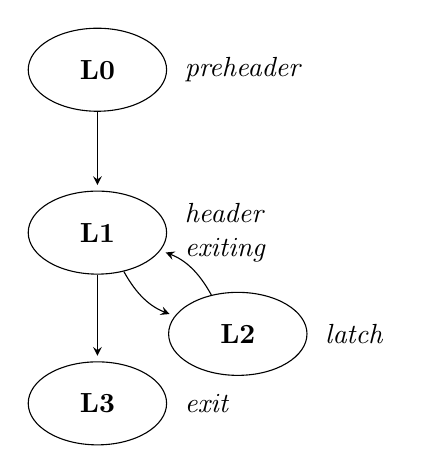
\begin{tikzpicture}[%
    ->,
    shorten >=2pt,
    >=stealth,
    node distance=.1cm,
    noname/.style={%
      ellipse,
      minimum width=5em,
      minimum height=3em,
      draw}
    ]
    \node[noname] (1) {\textbf{L0}};
    \node[noname] (2) [node distance=1cm,below=of 1] {\textbf{L1}};
    \node[noname] (4) [node distance=.75cm,below right=of 2] {\textbf{L2}};
    \node[noname] (6) [node distance=1.1cm,below=of 2] {\textbf{L3}};
    \path (1) edge node{} (2)
          (2) edge node{} (6)
          (2) edge [bend right=20pt] node{} (4)
          (4) edge [bend right=20pt] node {} (2);
    \node (7) [right=of 1] {\emph{preheader}};
    \node (7) [text width=6em,right=of 2] {\emph{header\\exiting}};
    \node (7) [right=of 4] {\emph{latch}};
    \node (7) [right=of 6] {\emph{exit}};
  \end{tikzpicture}
  \end{mdframed}
  \caption{CFG of a generic Loop}
  \label{fig:loopcfg}
\end{figure}

The \emph{Header} is the entrance block of the loop, the first to be executed. Every other block inside the loop is marked as \emph{Latch}. The \emph{Exiting} block is a block in the loop whose at least one successor is outside the loop. There are also two other elements that do not directly belong to the loop, but are needed to define it. The \emph{Preheader} block is any predecessor of the header block outside of the loop, and the \emph{Exit} block is any successor of the exiting block outside the loop.

\begin{figure}[t]
  \begin{mdframed}
  \centering
  \begin{subfigure}[b]{0.49\textwidth}
    \centering
    \begin{lstlisting}
define i32 @main(i32 %argc, i8** %argv) nounwind uwtable {
l0:
  %a = add i32 3, 0
  %b = add i32 2, 0
  br label %l1

l1:
  %i0 = phi i32 [ 1, %l0 ], [ %i1, %l2 ]
  %cmp = icmp sle i32 %i0, 100
  br i1 %cmp, label %l2, label %l3

l2:
  %c = add i32 %a, %b
  %i1 = add i32 %i0, %c
  br label %l1

l3:
  ret i32 0
}
    \end{lstlisting}
    \caption{Source}
    \label{fig:slicm}
  \end{subfigure}
  \begin{subfigure}[b]{0.49\textwidth}
    \centering
    \begin{lstlisting}
define i32 @main(i32 %argc, i8** %argv) nounwind uwtable {
l0:
  %a = add i32 3, 0
  %b = add i32 2, 0
  %c = add i32 %a, %b
  br label %l1

l1:
  %i0 = phi i32 [ 1, %l0 ], [ %i1, %l2 ]
  %cmp = icmp sle i32 %i0, 100
  br i1 %cmp, label %l2, label %l3

l2:
  %i1 = add i32 %i0, %c
  br label %l1

l3:
  ret i32 0
}
    \end{lstlisting}
    \caption{Target}
    \label{fig:tlicm}
  \end{subfigure}
  \end{mdframed}
  \caption[LOOP INVARIANT CODE MOTION EXAMPLE]{Loop invariant code motion example. The CFG of the loop is given in Figure~\ref{fig:loopcfg}}
  \label{fig:licm}
\end{figure}

Hoisting is possible when an instruction in the latch or header blocks uses only instructions that are in the preheaders of the loop (or in their predecessor) and the loop is guaranteed to execute at least once. In the example in Figure~\ref{fig:licm}, the instruction \texttt{\%c = add i32 \%a, \%b} is moved from the latch block \texttt{l2} to the preheader block \texttt{l0}. In LICM the witness is built in the following way: if a statement is moved from a loop block $B$ to the preheader block $H$, $B$ and $\bar{H}$ is put into relation with $B$, where the bar means, as usual a target location. Morover, the variable values are preserved ($\forall x \in V, x=\bar{x}$) , except for the variables that have assignment in these blocks.

The generated witness for this transformation may stutter, as LICM is a reordering transformation. In the example above, \texttt{l0} $\rightarrow$ \texttt{l1} $\rightarrow$ \texttt{l2} in the target stutters in \texttt{l0} in the source. This requires the witness checker to prove the correctness for the following formula:
\[
\begin{array}{l}
  \forall u \in I_B, \exists s \in I_B, X(u,s) \\
  \land \forall u,v \in S_B, s \in S_A, (X(u,s) \land R_B(U,V)) \implies( \\
  \hspace{1cm}(\exists t \in S_A, X(v,t) \land R_A(S,t))\\
  \hspace{1cm}\lor (\exists t \in S_A, X(u,t) \land R_A(S,t) \land X(u,s) \prec  X(u,t))\\
  \hspace{1cm}\lor (X(v,s) \land X(u,s) \prec  X(v,s)\\
  )
\end{array}
\]
As before, the universal quantifier is eliminated and the formula is negated before being discharged to the SMT solver.

The external annotations can be plugged to the \texttt{LoopInfo} class that takes track of all the invariants regarding a loop and is queried by the loop transformation during the analysis phase. Invariants can be explicitly injected in the LoopInfo with the method \texttt{makeLoopInvariant}.


% \chapter{Results}
% 		\label{cha:results}
% 		% !TEX root =  ../thesis.tex




\chapter{Results, Conclusions and Future Works}
	\label{cha:conclusions}
	% !TEX root =  ../thesis.tex

\section{Results}
\label{sec:results}

Based on the LLVM optimization framework, we were able to develop a program that has all the functionalities required in order to have a working annotation framework and a witness transformation system. The program was tested with several IR functions. The programs were written in C, converted to Intermediate Representation with CLANG, and a \texttt{mem2reg} pass was run to remove instruction types not processable by the ACSL transformations. The test cases have been uploaded to the repository.
The translator was able to fully translate from Intermediate Representation to a transition relation between either single instructions or basic blocks of instructions. The witness generator for Constant Propagation, Dead Code Elimination and Control Flow Graph Compression proved to be correct both with stuttering and step simulation. For testing purposes the transformations were slightly ``modified'' to be buggy; indeed, a correctness proof could not be generated. The generation and verification of the witness didn't suffer a considerable overhead of time w.r.t. their corresponding optimizations

\subsection{Times}
\label{sub:times}

To calculate the overhead incurred by Z3 for generate and verify the witness in general run, times were measured for different runs. The test cases were run in sequence and the tool \texttt{time-passes} of the LLVM optimizer was run together with different instances of the passes. For each test case and transformation, two runs were performed, one with the ACSL version of the pass, and one with the regular LLVM version. The run times were compared to calculate the overhead; Tables~\ref{tab:res1} and~\ref{tab:res2} show the results.

\begin{table}[t]
\centering
\begin{tabular}{|c|c|c|c|c|c|c|}
\hline
\multirow{3}{*}{} & \multicolumn{6}{c|}{Pass execution timing report (ms)} \tabularnewline
\cline{2-7}
 & \multicolumn{3}{c|}{Constant Propagation} & \multicolumn{3}{c|}{DCE + CFGC}\tabularnewline
\cline{2-7}
 & LLVM & ACSL & Diff & LLVM & ACSL & Diff\tabularnewline
\hline
\hline
Test 1 (11 LOC) & 1.1 & 14.1 & 13.0 & 0.5 & 9.2 & 7.7 \tabularnewline
\hline
Test 2 (28 LOC) & 1.2 & 49.7 & 48.5 & 0.4 & 18.3 & 17.9 \tabularnewline
\hline
Test 3 (28 LOC) & 1.0 & 54.8 & 53.8 & 1.2 & 40.1 & 38.9 \tabularnewline
\hline
Test 4 (10 LOC) & 1.1 & 16.0 & 14.9 & 0.4 & 8.8 & 8.4 \tabularnewline
\hline
Test 5 (96 LOC) & 1.5 & 445.3 & 443.8 & 1.0 & 106.9 & 105.9 \tabularnewline
\hline
Test 6 (37 LOC) & 1.1 & 116.5 & 115.3 & 0.8 & 88.3 & 86.5 \tabularnewline
\hline
Test 7 (24 LOC) & 1.1 & 27.2 & 26.1 & 0.4 & 25.5 & 25.1 \tabularnewline
\hline
Average & 1.01 & 103.37 & 101.36 & 0.67 & 42.38 & 41.71 \tabularnewline
\hline
\end{tabular}

\caption{RESULT TIMES FOR CONSTANT PROPAGATION, DCE AND CFGC}
\label{tab:res1}
\end{table}

\begin{table}[t]
\centering
\begin{tabular}{|c|c|c|c|c|c|c|}
\hline
\multirow{3}{*}{} & \multicolumn{3}{c|}{Pass execution timing report (ms)} \tabularnewline
\cline{2-4}
 & \multicolumn{3}{c|}{Loop Invariant Code Motion} \tabularnewline
\cline{2-4}
 & LLVM & ACSL & Diff\tabularnewline
\hline
\hline
Test 1 (24 LOC) & 0.1 & 49.6 & 49.5 \tabularnewline
\hline
Test 2 (130 LOC) & 0.5 & 340.5 & 340.5 \tabularnewline
\hline
Average & 0.3 & 200.06 & 200.03 \tabularnewline
\hline
\end{tabular}

\caption{RESULT TIMES FOR LOOP INVARIANT CODE MOTION}
\label{tab:res2}
\end{table}

Although the results show a considerable overhead on small samples, it appears to not grow linearly with the size of the code. Furthermore, the code can be analyzed to improve performance and tested for memory leakage and other implementation details, that are outside of the proof of concept that these results wanted to demonstrate.

\subsection{Issues}
\label{sub:issues}

The witness generator for Loop Invariant code motion showed some false positives, proving correct some incorrect transformations. This is due to the fact that LLVM loop analysis is deep and articulated, and an instruction can be moved for different reasons other than the ones that the witness is able to describe. The solution to the problem can be either to modify the witness generator to include all the case produced by LICM analysis, or to reduce the scope of the analysis and perform further optimization in a separate transformation pass.

The LLVM Annotation Framework presented here is still on developement phase and it will then be part of a bigger framework that handles how the external invariants are imported and fully exploited. This is a related work that goes beyond the scope of this work.

\section{Conclusions and Related Works}
\label{sub:related_works}
Showing the correctness of program transformations, in particular compiler optimizations, is a long-standing problem. There are numerous works that target specific compilers and languages. In  \cite{leroy2009formal}, Leroy gives a nice technical and historical view of approaches to this question. A first approach is that of verification: to formally prove each transformation correct, over all legal input programs. This is the approach taken, for example, by the CompCert project \cite{leroy2006formal}. However, formally verifying a full-fledged optimizing compiler, as one would verify any other large program, is practically infeasible, due mainly to the size of the code of the passes, evolution over time, and, possibly, proprietary considerations.

The \emph{Translation Validation} approach offers an alternative to the verification of translators in general and of compilers in particular. Using the translation validation approach, rather than verify the compiler itself one constructs a validating tool which, after every run of the compiler, formally confirms that the target code produced is a correct translation of the source program. The work in \cite{pnueli1998code} developed a tool for translation validation that succeeded in automatically verifying translations involving approximately 10,000 lines of source code in about 10 minutes. Its success critically depended on some simplifying assumptions that restrict the source and target to programs with a single external loop, and assumed a very limited set of optimizations. Subsequent approaches like the one in \cite{Rinard99crediblecompilation} considered translation validation for less restrictive languages, allowing, for example, nested loops. They also considered a more extensive set of optimizations. However, the methods proposed there were restricted to structure preserving optimizations. They could not directly deal with more aggressive optimizations such as loop distribution and loop tiling that are often used in more advanced optimizing compilers, nor could they handle simpler optimizations which relied on stuttering for correctness.

The approach presented offers similarity to translation validation, but it differs as it requires that the optimization is known and can be analyzed and modified. This gives the opportunity to add a witness generator which produces a different witness for every transformation that undergoes a generic program at compile time. This makes the witness approach, in principle, applicable to any optimization: stuttering simulation witnesses are proved to be complete and sound regardless of the transformation considered.

In practice, the real limitation is given by the possible high complexity that a witness can reach. The logics needed to express witness may not have decision procedures, so that fully automated checking is not possible. However, using SMT solvers, particullary Z3 in this context, it was possible to evaluate the witnesses expressed in this work. The complexity could also arise from the externally provided invariant, of which nothing can be known a priori. This can hamper the logics used by Z3 and result in situations were it couldn't be able to produce a result.

A solution for the problem of propagating invariants across transformations is also provided. This will be useful in the case where the annotations are given to the compiler so it could make use of them to perform further and better performing optimizations without having to improve the scope of the internal analysis. This problem had not been addressed in the general form discussed here.

Regarding formal verification works over the LLVM framework, LAV \cite{vujovsevic2012development} that statically checks program assertions and errors, and KLEE \cite{cadar2008klee}, capable of automatically generating tests that achieve high coverage on a diverse set of complex and environmentally-intensive programs.

\section{Future Works}
\label{sec:future_works}
The framework described in this work is at an early stage of implementation, and needs to be improved in several aspects and tested thoroughly. Even if the design and the basic structure has been implemented, in order for the project to be used in significant real case projects, some extensions are necessary.

The first important feature that needs to be expanded is the Intermediate Representation support. Currently the framework doesn't support store and load instructions to the memory and function calls. Including them in the witness generation and in the translator will require some non trivial modifications, especially for memory instructions. In fact, including them, means that the IR will not be a ``pruned'' SSA, and the generated invariants will need to be checked more carefully.

The framework can also be improved in other directions, for example by expanding the supported types with floats or charachters. Introducing pointer and arrays, though necessary for including real case scenarios, will need some effort, in order to correctly deal with aliasing issues. Certainly, several optimizations can be added to the framework, beginning from Conditional Contant Propagation and some Loop Reordering transformations, such as Loop Reversal, Interchange or Skewing Transformations.


	\clearpage
	\phantomsection
	\appendices
		\appendix \label{app:a}
		% !TEX root =  ../thesis.tex
\chapter{Brief program guide, instructions and examples}

These are the steps to correctly compile and use the framework.

\begin{enumerate}
  \item Download the repository from \url{https://bitbucket.org/itajaja/llvm-csfv}
  \item Compile and install Z3 following the instruction provided in the source code. In this work the version 4.3.1 of Z3 was used
  \item Compile LLVM running \texttt{make} in the project root folder
  \item (Optional) Install the LLVM executable with \texttt{make install}
  \item The Witness-augmented optimizations are in the folder \texttt{lib/Transforms/Acsl/witness/}. They are compiled separately and dinamically linked to the LLVM optimizer
  \item run \texttt{make} in the witness folder
  \item To run an ACSL pass over an IR file, run the following command
  \begin{center}
\texttt{\footnotesize <PROJECT\_FOLDER>/Debug+Asserts/bin/opt -load /usr/lib/libz3.so -load <PROJECT\_FOLDER>/Debug+Asserts/lib/Acsl.so -acslcp  <InputFile.s>}  \end{center}
where \emph{acslcp} can be substituted by any other optimization name.\\
To run an ACSL pass over a C program, run the following command
  \begin{center}
\texttt{\footnotesize <PROJECT\_FOLDER>/Debug+Asserts/bin/clang -load /usr/lib/libz3.so -load <PROJECT\_FOLDER>/Debug+Asserts/lib/Acsl.so -mem2reg -acslcp  <InputFile.c>}  \end{center}
\item To show debug strings, add the option \texttt{-debug-only='acsl'}
\item To add any other ACSL pass, follow the structure of the existing ones, the run \texttt{make} inside the witness folder
\end{enumerate}


	\clearpage
	\phantomsection
	\bib
	\bibliography{biblio}
	\nocite{*}

	\newpage
	\phantomsection

	% !TEX root =  ../thesis.tex

\vita

\begin{center}
\begin{singlespace}

\vspace{0.2in}

\begin{tabular}{r@{\hspace{0.2in}}|@{\hspace{0.2in}}p{4.5in}}

{\Large Education}
& \textbf{Bachelor of Science Degree in Engineering of Computing Systems} \\
& Politecnico di Milano \\
& 2008 - 2011 \\
\\
& \textbf{Master of Science Degree in Computer Science} \\
& University of Illinois at Chicago, Chicago, IL \\
& 2012 - 2013 \\
\\
& \textbf{Master of Science Degree in Engineering of Computing Systems} \\
& Politecnico di Milano, Politecnico di Torino \\
& 2011 - current \\
\\

{\Large Master thesis}
& \textbf{An Annotation Framework for the LLVM Compiler Infrastructure} \\
& Lenore Zuck, Professor (for reference, contact: \texttt{lenore@uic.edu}) \\
& \textbf{Topics}: Compilers, formal methods \\
\\

{\Large Technological skills}
& \textbf{Languages} \\
& Java, C\#, PHP, C \\
& \textbf{technologies} \\
& Andorid, Java EE, ASP.NET, OpenGL \\
& \textbf{Tools} \\
& \LaTeX, Git, SVN, Matlab \\
& \textbf{Databases} \\
& SQL family \\
& \textbf{OSs} \\
& Windows and Linux \\
\\
\end{tabular}


\newpage
\begin{tabular}{r@{\hspace{0.2in}}|@{\hspace{0.2in}}p{4.5in}}

{\Large Working Experience}
& \textbf{DARPA / University of Illinois} \\
& \emph{Research Assistant} \\
& 2012-2013 \\
& Employed in DARPA's CSFV (Crowd Sourced Formal Verification) Project.CSFV investigates extensions of compilers' optimizations using formal verification. \\
& Skills and technologies used:
\begin{itemize}
  \item C++
  \item Understanding and hacking of the LLVM-CLANG compiler infrastructure
  \item ACSL annotation language for C programs
  \item Z3 SMT solver
  \item OCaml
  \item Bison - Yacc
\end{itemize}
\\
& \textbf{Mark-Up Consulting Srl} \\
& Software Developer \\
& 2011-2012 \\
& Design, development, and maintenance of projects for business consulting and staff training.\\
& Skills and technologies used:
\begin{itemize}
  \item PHP development and deploy, using Moodle Framework
  \item Client-Server application development in C\#:
  \begin{itemize}
    \item WPF - Windows Presentation Framework
    \item WCF - Windows Communication Framework
  \end{itemize}
  \item MySql and SQLite Databases
\end{itemize}
\\
\end{tabular}
\end{singlespace}
\end{center}


\end{document}
